% Options for packages loaded elsewhere
\PassOptionsToPackage{unicode}{hyperref}
\PassOptionsToPackage{hyphens}{url}
\PassOptionsToPackage{dvipsnames,svgnames,x11names}{xcolor}
\documentclass[
  11pt,
]{article}
\usepackage{xcolor}
\usepackage[a4paper, margin=2.4cm]{geometry}
\usepackage{amsmath,amssymb}
\setcounter{secnumdepth}{-\maxdimen} % remove section numbering
\usepackage{iftex}
\ifPDFTeX
  \usepackage[T1]{fontenc}
  \usepackage[utf8]{inputenc}
  \usepackage{textcomp} % provide euro and other symbols
\else % if luatex or xetex
  \usepackage{unicode-math} % this also loads fontspec
  \defaultfontfeatures{Scale=MatchLowercase}
  \defaultfontfeatures[\rmfamily]{Ligatures=TeX,Scale=1}
\fi
\usepackage{lmodern}
\ifPDFTeX\else
  % xetex/luatex font selection
\fi
% Use upquote if available, for straight quotes in verbatim environments
\IfFileExists{upquote.sty}{\usepackage{upquote}}{}
\IfFileExists{microtype.sty}{% use microtype if available
  \usepackage[]{microtype}
  \UseMicrotypeSet[protrusion]{basicmath} % disable protrusion for tt fonts
}{}
\makeatletter
\@ifundefined{KOMAClassName}{% if non-KOMA class
  \IfFileExists{parskip.sty}{%
    \usepackage{parskip}
  }{% else
    \setlength{\parindent}{0pt}
    \setlength{\parskip}{6pt plus 2pt minus 1pt}}
}{% if KOMA class
  \KOMAoptions{parskip=half}}
\makeatother
\usepackage{longtable,booktabs,array}
\newcounter{none} % for unnumbered tables
\usepackage{calc} % for calculating minipage widths
% Correct order of tables after \paragraph or \subparagraph
\usepackage{etoolbox}
\makeatletter
\patchcmd\longtable{\par}{\if@noskipsec\mbox{}\fi\par}{}{}
\makeatother
% Allow footnotes in longtable head/foot
\IfFileExists{footnotehyper.sty}{\usepackage{footnotehyper}}{\usepackage{footnote}}
\makesavenoteenv{longtable}
\usepackage{graphicx}
\makeatletter
\newsavebox\pandoc@box
\newcommand*\pandocbounded[1]{% scales image to fit in text height/width
  \sbox\pandoc@box{#1}%
  \Gscale@div\@tempa{\textheight}{\dimexpr\ht\pandoc@box+\dp\pandoc@box\relax}%
  \Gscale@div\@tempb{\linewidth}{\wd\pandoc@box}%
  \ifdim\@tempb\p@<\@tempa\p@\let\@tempa\@tempb\fi% select the smaller of both
  \ifdim\@tempa\p@<\p@\scalebox{\@tempa}{\usebox\pandoc@box}%
  \else\usebox{\pandoc@box}%
  \fi%
}
% Set default figure placement to htbp
\def\fps@figure{htbp}
\makeatother
\setlength{\emergencystretch}{3em} % prevent overfull lines
\providecommand{\tightlist}{%
  \setlength{\itemsep}{0pt}\setlength{\parskip}{0pt}}
\usepackage{amsmath,amssymb,amsthm}
\usepackage{booktabs,longtable}
\usepackage{xurl}
\setlength{\emergencystretch}{3em}
\usepackage{bookmark}
\IfFileExists{xurl.sty}{\usepackage{xurl}}{} % add URL line breaks if available
\urlstyle{same}
\hypersetup{
  pdftitle={No Szöllősi matrix lies in a quadruplet of mutually unbiased bases in dimension six: a certificate replayed by an independent checker{,} with a rigorous re-proof for the Fourier family},
  pdfauthor={Anonymous},
  colorlinks=true,
  linkcolor={blue},
  filecolor={Maroon},
  citecolor={Blue},
  urlcolor={blue},
  pdfcreator={LaTeX via pandoc}}

\title{No Szöllősi matrix lies in a quadruplet of mutually unbiased
bases in dimension six: a certificate replayed by an independent
checker, with a rigorous re-proof for the Fourier family}
\author{Anonymous}
\date{30 September 2026}

\begin{document}
\maketitle

\section{Abstract}\label{abstract}

Matolcsi, Matszangosz, Varga and Weiner (MMVW, 2026) reduced Zauner's
conjecture --- that \(\mathbb C^6\) carries at most three mutually
unbiased bases (MUBs) --- to an algebraic identity for MUB triplets
(their Conjecture 2) together with their Conjecture 3: no complex
Hadamard matrix in Szöllősi's two-circulant family \(X(\alpha)\) is part
of a quadruplet of MUBs. They remarked that Conjecture 3 should be
provable with the discretisation technique of Jaming, Matolcsi, Móra,
Szöllősi and Weiner (2009), ``although the actual implementation could
be tedious''. We prove Conjecture 3 for the whole closed parameter
region, boundary and degenerate loci included.

The proof is a computer-assisted certificate with a deliberately split
architecture. An untrusted \emph{generator} covers a fundamental domain
of the family's symmetry group by 14,658 parameter boxes and, for each
box, produces a finite family of phase-space boxes (``hulls'') intended
to contain every vector unbiased to both the standard basis and the
Hadamard basis, for every parameter in the box. A separate
\emph{checker}, which shares no code with the generator, then replays
every certificate: its trusted kernel (638 lines of C) moves every
floating-point result one unit in the last place outward, uses no
library transcendental function, and decides by exhaustive branch and
bound (with a modulus test, a mean-value test and a parametric Krawczyk
test) that the hulls cover all unbiased vectors; it then recomputes the
orthogonality and unbiasedness graphs of the hulls and shows, by its own
clique search, that no two further mutually unbiased bases fit into
them. The checker also re-derives the parameter cover with its own
selector. All 14,658 certificates were verified, 75 of them after
subdividing their parameter boxes.

The same interface was applied to the two-parameter Fourier family
\(F(a,b)\). Exact symmetry and tiling checks justify its fundamental
triangle, and 1,935 certificates give a new implementation of the
exclusion already proved by Jaming et al.~(2009), not a new Fourier
exclusion theorem. The general dimension-six maximum remains conditional
on MMVW's Conjecture 2. ``Independent checker'' refers to separation
from the generator, not external peer review or proof-assistant
formalisation.

\section{1. Introduction}\label{introduction}

\subsection{1.1 The problem}\label{the-problem}

Two orthonormal bases \(\{e_k\}\) and \(\{f_l\}\) of \(\mathbb C^d\) are
\emph{mutually unbiased} if \(|\langle e_k,f_l\rangle|^2=1/d\) for all
\(k,l\). If the bases are the columns of unitary matrices \(X_1,X_2\),
the condition says that \(\sqrt d\,X_1^*X_2\) is a \emph{complex
Hadamard matrix}: a matrix with unimodular entries whose columns are
orthogonal. In prime-power dimensions there are \(d+1\) mutually
unbiased bases; in dimension six the largest known sets have three
members, and Zauner's conjecture (Zauner 2011) asserts that three is the
maximum. The question is the best-known open case of the MUB problem and
has resisted analytic, numerical and algebraic attacks for more than two
decades (McNulty and Weigert 2026 give a recent review).

By a unitary change of basis any set of MUBs can be brought into a form
in which the first basis is the standard basis (\(X_1=I\)) and the
second is \(H/\sqrt6\) for a complex Hadamard matrix \(H\). Every
further basis consists of unit vectors unbiased to both. Up to a phase,
the vectors unbiased to \(I\) are \(v(\theta)/\sqrt6\) with
\(v(\theta)=(1,e^{i\theta_2},\dots,e^{i\theta_6})^{\mathsf T}\), and
unbiasedness to \(H/\sqrt6\) becomes a system of trigonometric equations
in \(\theta\in\mathbb T^5\) whose solution set we denote by
\(\mathcal U(H)\). A quadruplet \(\{I,H/\sqrt6,C,D\}\) exists exactly
when \(\mathcal U(H)\) contains two orthonormal bases that are unbiased
to each other.

MMVW (2026) studied MUB triplets through their transition matrices and
showed that one algebraic identity (their Conjecture 2) forces every
Hadamard matrix occurring in a triplet to lie in one of two families:
the two-parameter Fourier family \(F(a,b)\), which Jaming et al.~(2009)
had shown cannot be extended to a quadruplet, and Szöllősi's
two-parameter family \(X(\alpha)\) (Szöllősi 2010). For the latter they
stated:

\begin{quote}
\textbf{Conjecture 3 (MMVW).} Any matrix \(S\in X(\alpha)\) in the
Szöllősi family, defined in (4.2), cannot be part of an MUB-quadruplet.
In principle, this conjecture can be proven with the discretization
technique in {[}Jaming et al.~2009{]}, although the actual
implementation could be tedious.
\end{quote}

An earlier claim of this statement, derived from a lemma of Chen, Liang,
Hu and Chen (2021), is not secure: McNulty and Weigert (2025) identified
a defect in the underlying argument, and the reply of Liang and Chen
(2025) does not restore it. The display (4.2) of MMVW is Szöllősi's
two-circulant form \[
S=\begin{bmatrix} A&B\\ B^*&-A^*\end{bmatrix},\qquad A=\mathrm{circ}(a,b,c),\quad B=\mathrm{circ}(d,e,f),\qquad |a|=\dots=|f|=1 ,
\] and \(X(\alpha)\) denotes the complex Hadamard matrices of this form,
which up to equivalence are parametrised by a complex number \(\alpha\)
in a closed region \(\mathbb D\) bounded by arcs of a deltoid and its
negative (Section 3).

\subsection{1.2 Results}\label{results}

\begin{quote}
\textbf{Theorem 1.} Let \(S\) be a complex Hadamard matrix of order six
of the form (4.2). There are no unitary matrices \(C,D\) such that
\(\{I,S/\sqrt6,C,D\}\) is a set of four mutually unbiased bases of
\(\mathbb C^6\). Equivalently, no member of \(X(\alpha)\), for any
\(\alpha\in\mathbb D\) including the boundary, is part of an MUB
quadruplet.
\end{quote}

\begin{quote}
\textbf{Corollary 2.} If Conjecture 2 of MMVW holds, then the maximal
number of mutually unbiased bases in \(\mathbb C^6\) is three.
\end{quote}

The corollary is Proposition 4.2 of MMVW with Conjecture 3 discharged by
Theorem 1; the Fourier half of their argument rests on Jaming et
al.~(2009), which we re-prove:

\begin{quote}
\textbf{Theorem 3 (Jaming, Matolcsi, Móra, Szöllősi and Weiner 2009,
Theorem 1.4).} For no \((a,b)\in[0,1)^2\) can the pair \(\{I,F(a,b)\}\)
be extended to a quadruplet of mutually unbiased bases.
\end{quote}

Theorem 3 is not new. We supply a separated checker and inspectable
certificates for the published Fourier exclusion. No
implementation-specific criticism of the historical software is needed
for this contribution. Fourier also tests transfer between the two
implemented families: they share a checker and certificate format, with
family-specific exponent data, coefficient rectangles and selectors.
Extensions beyond these families remain future work.

\subsection{1.3 What is new, and how it relates to Jaming et
al.}\label{what-is-new-and-how-it-relates-to-jaming-et-al.}

The overall strategy --- cover the parameter space by cells, enclose the
unbiased vectors for each cell, and exclude quadruplets combinatorially
--- is that of Jaming et al.~(2009), and MMVW explicitly anticipated its
use for Conjecture 3. The contributions of this paper are the following.

\begin{enumerate}
\def\labelenumi{\arabic{enumi}.}
\tightlist
\item
  \emph{The theorem.} Theorem 1 is new; it removes one of the two
  remaining hypotheses in MMVW's route to Zauner's conjecture.
\item
  \emph{A family-level certificate interface} (Section 2): an
  \emph{admissible family} is specified by integer exponent vectors,
  unimodular coefficients and an optional trigonometric constraint; a
  \emph{certificate} for a parameter box is a list of hulls in the phase
  torus; and four proof obligations (selector soundness, coverage,
  self-separation of hulls, and a clique condition) imply, for every
  fundamental-domain parameter in its ownership cell, that the Hadamard
  matrix is not part of a quadruplet. Closed boxes supply the interval
  enclosures; half-open cells supply ownership. The interface is what
  made the Fourier family a change of input data rather than a new
  program.
\item
  \emph{Treatment of degenerate parameters without isolating roots.}
  Along the ray \(\arg\alpha=\pi/6\) and near \(\alpha=0\) unbiased
  vectors coalesce (Section 10). Jaming et al.~separated vectors with a
  fixed-resolution grid; methods that isolate simple roots fail near
  coalescence at any fixed resolution. Here the exclusion of phase boxes
  is driven by a \emph{parametric} Krawczyk operator acting uniformly
  over a parameter box, and hulls are allowed to contain clusters of
  solutions; the combinatorial step only needs the hulls to be small
  enough for the self-separation condition.
\item
  \emph{A verification design with an explicit trusted computing base}
  (Sections 5--8). The generator is untrusted. The checker re-derives
  the owner cover, re-verifies phase-space coverage, and recomputes the
  graph exclusion using outward-rounded intervals. The test suite
  detects 16 of 17 supplied kernel mutations; that is substantial but
  incomplete mutation coverage. Section 8 states the surviving mutation
  and the additional exact generic mixed-term fixture without claiming
  exhaustive testing.
\end{enumerate}

\subsection{1.4 History of this work}\label{history-of-this-work}

The supplied first review reproduced counterexamples to the earlier
generator's radius arithmetic, cyclic hulls and resumption logic, and
identified an uncertified selector margin. The version-2 package
introduced a separate checker and new certificates. The supplied second
review then identified the closed-box ownership mismatch and an
input-unbound replay cache. This revision repairs those contracts and
withdraws the unused generator-rounding argument. Neither review
demonstrated a false exclusion theorem. Review provenance is not
independently authenticated, and no external human peer review is
asserted. Appendix B records the second-review dispositions; historical
records remain distinct from the new clean replay.

\subsection{1.5 Organisation}\label{organisation}

Section 2 sets up admissible families, the quadruplet property and the
certificate, and states the proof obligations. Sections 3 and 4 treat
the Szöllősi and Fourier families: parametrisation, exact symmetries,
fundamental domains and selectors. Section 5 describes the checker's
arithmetic and Section 6 its exclusion tests and coverage verification.
Section 7 describes the generator. Section 8 describes the verification
architecture, the trusted computing base and the tests. Section 9
reports the computations and Section 10 some numerical diagnostics of
degenerate parameters, which are not part of the proof. Section 11
discusses scope and limitations.

\section{2. Families, certificates and proof
obligations}\label{families-certificates-and-proof-obligations}

\subsection{2.1 Admissible families}\label{admissible-families}

Write \(\mathbb T=\mathbb R/2\pi\mathbb Z\). An \emph{admissible family}
of order six with \(m\) parameters consists of

\begin{itemize}
\tightlist
\item
  integer exponent vectors \(E_{kj}\in\mathbb Z^m\) and unimodular
  constants \(c_{kj}\) (\(1\le k,j\le6\)), defining \[
  H(p)_{kj}=c_{kj}\,e^{i\langle E_{kj},p\rangle},\qquad p\in\mathbb T^m ;
  \]
\item
  optionally, a \emph{constraint}
  \(C(p)=\sum_{t}\gamma_t\,e^{i\langle e_t,p\rangle}\) with integer
  vectors \(e_t\) and constants \(\gamma_t\), whose zero set
  \(\Sigma=\{p: C(p)=0\}\) is the set of parameters at which \(H(p)\) is
  a complex Hadamard matrix (without a constraint,
  \(\Sigma=\mathbb T^m\) and \(H(p)\) must be Hadamard for all \(p\));
\item
  a \emph{fundamental domain} \(\mathcal F\subseteq\Sigma\) with the
  property that the quadruplet question for every \(p\in\Sigma\) reduces
  to the same question for some point of \(\mathcal F\) (Sections 3.3
  and 4.3), together with a \emph{selector} that retains the canonical
  half-open dyadic owner of every point of \(\mathcal F\) at every
  relevant level.
\end{itemize}

Use representatives in \([0,2\pi)^m\) and define
\[Q_{\ell,i}=\prod_r[2\pi i_r/2^\ell,2\pi(i_r+1)/2^\ell),\qquad P_{\ell,i}=\overline{Q_{\ell,i}}.\]
Closure is on the torus; the endpoint \(2\pi\) is represented by \(0\)
for ownership. Each point has a unique owner at each level, and its
finer owner is a child of its coarser owner. Closed enclosures are used
for interval calculations. A discarded enclosure may meet \(\mathcal F\)
on a shared boundary.

For the Szöllősi family \(m=4\), all \(c_{kj}=\pm1\), and the constraint
has six terms (Section 3). For the Fourier family \(m=2\), the
\(c_{kj}\) are sixth roots of unity, and there is no constraint (Section
4). The checker consumes exactly this data: the exponent arrays,
rectangles enclosing the constants, and the selector.

\subsection{2.2 The quadruplet property}\label{the-quadruplet-property}

For a complex Hadamard matrix \(H\) of order six let \(\mathcal E(H)\)
be the statement: \emph{there exist unitary \(C,D\) such that
\(\{I,H/\sqrt6,C,D\}\) is a set of four mutually unbiased bases.} Two
Hadamard matrices are \emph{equivalent} if \(H'=M_1HM_2\) with monomial
unitary matrices \(M_1,M_2\) (products of a permutation matrix and a
diagonal unitary matrix).

\textbf{Lemma 4.} (i) If \(H'\) is equivalent to \(H\) then
\(\mathcal E(H)\iff\mathcal E(H')\). (ii)
\(\mathcal E(H)\iff\mathcal E(\overline H)\). (iii)
\(\mathcal E(H)\iff\mathcal E(H^*)\), hence
\(\mathcal E(H)\iff\mathcal E(H^{\mathsf T})\).

\emph{Proof.} (i) Let \(\{I,M_1HM_2/\sqrt6,C,D\}\) be a quadruplet.
Multiplying all four unitaries on the left by \(M_1^{-1}\) preserves
mutual unbiasedness and gives
\(\{M_1^{-1},HM_2/\sqrt6,M_1^{-1}C,M_1^{-1}D\}\). The columns of the
monomial unitary \(M_1^{-1}\) are the standard basis vectors up to
phases, and the columns of \(HM_2\) are those of \(H\) up to order and
phases; as bases these are \(I\) and \(H/\sqrt6\). The converse is the
same argument with \(M_1^{-1},M_2^{-1}\). (ii) Conjugate all four
matrices; conjugation is an involution. (iii) Put \(U=H/\sqrt6\) and let
\(\{I,U,C,D\}\) be a quadruplet. Then \(\{I,U^*,U^*C,U^*D\}\) is one:
\(U^*\), \(U^*C\), \(U^*D\) have entries of modulus \(1/\sqrt6\) because
\(U\) is unbiased to \(I\), \(C\) and \(D\); \((U^*)^*(U^*C)=C\) and
\((U^*)^*(U^*D)=D\) are unbiased to \(I\); and \((U^*C)^*(U^*D)=C^*D\)
is unbiased because \(C\) and \(D\) are. Since \((H^*)^*=H\) this is an
equivalence, and \(H^{\mathsf T}=\overline{H^*}\) with (ii) gives the
last claim. \(\square\)

\subsection{2.3 Unbiased vectors}\label{unbiased-vectors}

For a complex Hadamard matrix \(H\) and
\(\theta=(\theta_2,\dots,\theta_6)\in\mathbb T^5\) put
\(v(\theta)=(1,e^{i\theta_2},\dots,e^{i\theta_6})^{\mathsf T}\) and \[
S_j(\theta)=(H^*v(\theta))_j=\sum_{k=1}^6\overline{H_{kj}}\,v_k(\theta),\qquad j=1,\dots,6 .
\] The unit vector \(v(\theta)/\sqrt6\) is unbiased to the columns of
\(H/\sqrt6\) if and only if \(|S_j(\theta)|^2=6\) for all \(j\). Let \[
\mathcal U(H)=\{\theta\in\mathbb T^5:\ |S_j(\theta)|^2=6,\ j=1,\dots,6\}.
\] (For a Hadamard matrix \(\sum_j|S_j|^2=\|H^*v\|^2=36\), so one of the
six equations is implied by the others; the tests of Section 6 use
either all six or five of them, which is legitimate because a necessary
condition for membership in \(\mathcal U(H)\) is used to exclude.) No
finiteness of \(\mathcal U(H)\) is assumed anywhere.

\textbf{Lemma 5.} If \(\mathcal E(H)\) holds, there are twelve distinct
points \(\theta^{(1)},\dots,\theta^{(12)}\in\mathcal U(H)\) such that
\(\langle v(\theta^{(a)}),v(\theta^{(b)})\rangle=0\) for \(a\ne b\) both
in \(\{1,\dots,6\}\) or both in \(\{7,\dots,12\}\), and
\(|\langle v(\theta^{(a)}),v(\theta^{(b)})\rangle|^2=6\) for
\(a\le6<b\).

\emph{Proof.} Each column of \(C\) and of \(D\) is unbiased to \(I\), so
all its entries have modulus \(1/\sqrt6\). Multiplying a column by a
unimodular phase changes neither orthogonality within its basis nor
unbiasedness to other bases; after such a phase and the factor
\(\sqrt6\) the column is \(v(\theta)\) with \(\theta\in\mathcal U(H)\).
Orthogonality within \(C\) and \(D\) gives the zero inner products, and
unbiasedness of \(C\) and \(D\), \(|\langle c_a,d_b\rangle|^2=1/6\) for
unit vectors, becomes \(|\langle v,w\rangle|^2=6\) after rescaling by
\(\sqrt6\) each. Two of the twelve points coincide only if
\(|\langle v,v\rangle|^2=36\) equals \(0\) or \(6\), which is
impossible. \(\square\)

\subsection{2.4 Hulls and the combinatorial
certificate}\label{hulls-and-the-combinatorial-certificate}

A \emph{hull} is a box
\(\prod_{k=2}^{6}[l_k,h_k]\cdot\frac{2\pi}{2^{16}}\) in the phase torus
with integer end-points \(l_k\le h_k\) (if \(h_k-l_k\ge2^{16}\) the
factor is the whole circle). For hulls \(\mathsf h,\mathsf h'\) let
\(\Pi(\mathsf h,\mathsf h')\subseteq[0,\infty)\) be an interval
containing \(|\langle v(\theta),v(\phi)\rangle|^2\) for all
\(\theta\in\mathsf h\), \(\phi\in\mathsf h'\), and
\(\Pi(\mathsf h,\mathsf h)\) one containing these values for all
\(\theta,\phi\in\mathsf h\). Define two graphs on a finite family
\(\mathcal H\) of hulls: \[
\mathsf h\sim_O\mathsf h'\iff \mathsf h\ne\mathsf h',\ 0\in\Pi(\mathsf h,\mathsf h'),\qquad \mathsf h\sim_B\mathsf h'\iff \mathsf h\ne\mathsf h',\ 6\in\Pi(\mathsf h,\mathsf h').
\]

\textbf{Proposition 6 (combinatorial certificate).} Let \(H\) be a
complex Hadamard matrix and \(\mathcal H\) a finite family of hulls such
that

\begin{itemize}
\tightlist
\item
  (Cov)
  \(\mathcal U(H)\subseteq\bigcup_{\mathsf h\in\mathcal H}\mathsf h\);
\item
  (Sep) \(\Pi(\mathsf h,\mathsf h)\subset(6,\infty)\) for every
  \(\mathsf h\in\mathcal H\);
\item
  (Cl) there are no two six-cliques \(K_1,K_2\) of the graph \(O\) such
  that every pair in \(K_1\times K_2\) is an edge of \(B\).
\end{itemize}

Then \(\mathcal E(H)\) fails.

\emph{Proof.} Suppose \(\mathcal E(H)\) holds, take the twelve points of
Lemma 5 and assign to each a hull containing it (Cov). For two distinct
points of the twelve, \(|\langle v,w\rangle|^2\in\{0,6\}\); by (Sep)
they cannot share a hull, so the twelve hulls are distinct. The six
hulls of the first basis are pairwise joined in \(O\), likewise those of
the second basis, and every cross pair is joined in \(B\) (by the
definition of \(\Pi\)). This contradicts (Cl). \(\square\)

The certificate is \emph{uniform in the parameter}: if (Cov) holds for
\(H(p)\) for every \(p\) in a set \(P'\), and (Sep) and (Cl) hold for
the hull family (they do not involve \(p\)), then \(\mathcal E(H(p))\)
fails for every \(p\in P'\).

\subsection{2.5 Proof obligations}\label{proof-obligations}

A \emph{certificate} for a closed dyadic parameter box \(P\) is a finite
hull family \(\mathcal H_P\). A \emph{cover} is a set of certified
boxes. The following statement is what the checker establishes.

\textbf{Theorem 7.} Let an admissible family with fundamental domain
\(\mathcal F\) and selector be given, and a cover with certificates
\(\mathcal H_P\). Suppose

\begin{itemize}
\tightlist
\item
  (O1) \emph{selector soundness and cover completeness:} every kept cell
  of the selector's cover tree (Section 6.5) is either certified or has
  all its kept children covered, down to a finite depth; every
  \(p\in\mathcal F\) has its canonical owner retained at each relevant
  level;
\item
  (O2) \emph{coverage:} for every certified ownership cell \(Q\) with
  enclosure \(P\) and every \(p\in\mathcal F\cap Q\),
  \(\mathcal U(H(p))\subseteq\bigcup\mathcal H_P\);
\item
  (O3) \emph{separation:} (Sep) holds for every hull of every
  \(\mathcal H_P\);
\item
  (O4) \emph{clique condition:} (Cl) holds for every \(\mathcal H_P\).
\end{itemize}

Then \(\mathcal E(H(p))\) fails for every \(p\in\mathcal F\), and hence,
by the defining property of \(\mathcal F\), for every \(p\in\Sigma\).

\emph{Proof.} Follow the unique owners of \(p\in\mathcal F\) from the
top level. By (O1) they are retained, nested, and reach a certified cell
\(Q\) at finite depth. Thus \(p\in\mathcal F\cap Q\), and (O2)--(O4)
give Proposition 6 with \(\mathcal H=\mathcal H_P\). \(\square\)

In the Szöllősi case the reduction from \(\Sigma\) to \(\mathcal F\) is
Proposition 10, and every normalised matrix of the form (4.2) is
\(H(p)\) for some \(p\in\Sigma\) (Lemma 8); together these give Theorem
1. In the Fourier case the reduction is Proposition 12, which gives
Theorem 3.

\section{3. The Szöllősi family}\label{the-szuxf6llux151si-family}

\subsection{3.1 Normal form and
parameters}\label{normal-form-and-parameters}

Throughout, \(\mathrm{circ}(a_0,a_1,a_2)\) is the \(3\times3\) circulant
with rows \((a_0,a_1,a_2)\), \((a_2,a_0,a_1)\), \((a_1,a_2,a_0)\).
Circulants commute, are normal, and
\(\mathrm{circ}(a_0,a_1,a_2)^{\mathsf T}=\mathrm{circ}(a_0,a_2,a_1)\).

\textbf{Lemma 8 (normalisation and the Hadamard condition).} (i)
Multiplying rows \(1\)--\(3\) of \(S\) in (4.2) by \(\lambda\) and rows
\(4\)--\(6\) by \(\bar\lambda\), or columns \(1\)--\(3\) by \(\mu\) and
columns \(4\)--\(6\) by \(\bar\mu\) (\(|\lambda|=|\mu|=1\)), gives again
a matrix of the form (4.2), with \((A,B)\) replaced by
\((\lambda\mu A,\lambda\bar\mu B)\); consequently every matrix of the
form (4.2) is equivalent to one with \(a=d=1\). (ii) A matrix of the
form (4.2) with \(a=d=1\) is a complex Hadamard matrix if and only if
\(\bar b+b\bar c+c+\bar e+e\bar f+f=0\).

\emph{Proof.} (i) The scaled matrix is
\(\begin{bmatrix}\lambda\mu A&\lambda\bar\mu B\\ \bar\lambda\mu B^*&-\bar\lambda\bar\mu A^*\end{bmatrix}\),
and \((\lambda\bar\mu B)^*=\bar\lambda\mu B^*\),
\((\lambda\mu A)^*=\bar\lambda\bar\mu A^*\). Choosing
\(\lambda^2=\bar a\bar d\) and \(\mu=\bar a/\lambda\) gives
\(\lambda\mu=\bar a\), \(\lambda\bar\mu=\bar d\). (ii) Since \(A,B\) are
circulant, \(SS^*=\mathrm{diag}(AA^*+BB^*,\,B^*B+A^*A)\) and
\(A^*A=AA^*\), \(B^*B=BB^*\). \(AA^*\) is the circulant whose first row
is the autocorrelation of \((1,b,c)\), namely
\((3,\ \bar b+b\bar c+c,\ \overline{\bar b+b\bar c+c})\), and likewise
for \(B\). Hence \(SS^*=6I\) if and only if the stated sum vanishes.
\(\square\)

For \(p=(\theta_x,\theta_y,\theta_u,\theta_v)\in\mathbb T^4\) put \[
x=e^{i\theta_x},\ y=e^{i\theta_y},\ z=\overline{xy},\qquad u=e^{i\theta_u},\ v=e^{i\theta_v},\ w=\overline{uv},
\] \[
A(p)=\mathrm{circ}(1,\bar x,z),\quad B(p)=\mathrm{circ}(1,\bar u,w),\qquad H(p)=\begin{bmatrix}A(p)&B(p)\\ B(p)^*&-A(p)^*\end{bmatrix}.
\] This is (4.2) with \(a=d=1\), \(b=\bar x\), \(c=z\), \(e=\bar u\),
\(f=w\), and every unimodular \((b,c,e,f)\) arises (\(x=\bar b\),
\(y=b\bar c\), \(u=\bar e\), \(v=e\bar f\)). In these variables
\(\bar b+b\bar c+c=x+y+z\), so by Lemma 8 \(H(p)\) is Hadamard if and
only if \[
C(p):=x+y+z+u+v+w=0. \tag{C}
\] The family is admissible in the sense of Section 2.1: every entry of
\(H(p)\) is \(\pm e^{i\langle E,p\rangle}\) with \(E\in\{-1,0,1\}^4\)
having at most two non-zero entries, and \(C\) has six terms. An exact
symbolic computation (\texttt{exact/lemma5\_exact.py}, SymPy, treating
\(x,y,u,v\) as Laurent variables with \(\bar x=1/x\)) confirms that
every diagonal entry of \(H(p)H(p)^*\) is \(6\) and every off-diagonal
entry is \(0\), \(C(p)\) or \(\overline{C(p)}\), identically in \(p\).

\emph{Relation to Szöllősi's parameter.} Put \(\alpha=x+y+z\). Since
\(xyz=1\) and \(|x|=|y|=|z|=1\), \(xy+yz+zx=\bar\alpha\), so \(x,y,z\)
are the roots of \(f_\alpha(t)=t^3-\alpha t^2+\bar\alpha t-1\), and on
\(\Sigma\) the numbers \(u,v,w\) are the roots of \(f_{-\alpha}\).
Szöllősi's region is
\(\mathbb D=\{\alpha: D[\alpha]\le0,\ D[-\alpha]\le0\}\) with
\(D[\alpha]=|\alpha|^4+18|\alpha|^2-8\,\mathrm{Re}(\alpha^3)-27\), the
condition for \(f_\alpha\) to have three unimodular roots (Szöllősi
2010, Section 3). Conversely, for \(\alpha\in\mathbb D\) every labelling
of the roots of \(f_\alpha\) as \((x,y,z)\) and of \(f_{-\alpha}\) as
\((u,v,w)\) gives a point of \(\Sigma\). Thus \(\Sigma\) is precisely
the set of normalised matrices of the family for all \(\alpha\) in the
\emph{closed} region \(\mathbb D\) and all labellings; points on the
boundary of \(\mathbb D\), where roots coincide, are points of
\(\Sigma\) like any others and need no separate treatment.

\subsection{3.2 Symmetries}\label{symmetries}

Let \(\Pi=\mathrm{circ}(0,1,0)\), let \(P_{23}\) exchange indices \(2\)
and \(3\), \(D_\omega=\mathrm{diag}(1,\omega,\omega^2)\) with
\(\omega=e^{2\pi i/3}\), and write \(M_1\oplus M_2\) for a
block-diagonal matrix. Define the following maps of \(\mathbb T^4\),
written through the six unimodular numbers \((x,y,z,u,v,w)\), which
determine \(p\): \[
\begin{aligned}
\sigma_1&:(x,y,z,u,v,w)\mapsto(y,z,x,u,v,w), & \sigma_2&:(x,y,z,u,v,w)\mapsto(x,y,z,v,w,u),\\
\rho&:(x,y,z,u,v,w)\mapsto(\bar z,\bar y,\bar x,\bar w,\bar v,\bar u), & \tau&:(x,y,z,u,v,w)\mapsto(\bar z,\bar y,\bar x,\bar u,\bar v,\bar w),\\
\kappa&:(x,y,z,u,v,w)\mapsto(\bar x,\bar y,\bar z,\bar u,\bar v,\bar w), & \omega_\cdot&:(x,y,z,u,v,w)\mapsto\omega\,(x,y,z,u,v,w),\\
\varsigma&:(x,y,z,u,v,w)\mapsto(u,v,w,x,y,z). &&
\end{aligned}
\]

\textbf{Lemma 9 (matrix identities).} For every \(p\in\mathbb T^4\):

\begin{enumerate}
\def\labelenumi{\arabic{enumi}.}
\tightlist
\item
  \(H(\tau p)=H(p)^{\mathsf T}\);
\item
  \(H(\kappa p)=\overline{H(p)}\);
\item
  \(H(\rho p)=(P_{23}\oplus P_{23})\,H(p)\,(P_{23}\oplus P_{23})\);
\item
  \(H(\omega_\cdot p)=(D_\omega\oplus D_\omega)\,H(p)\,(D_\omega\oplus D_\omega)^{-1}\);
\item
  \(H(\varsigma p)=(I\oplus(-I))\,H(p)\,\begin{bmatrix}0&I\\I&0\end{bmatrix}\);
\item
  \(H(\sigma_1p)=(xI\oplus\Pi)\,H(p)\,(\Pi^{\mathsf T}\oplus\bar xI)\)
  and
  \(H(\sigma_2p)=(uI\oplus\Pi)\,H(p)\,(\bar uI\oplus\Pi^{\mathsf T})\).
\end{enumerate}

Moreover \(C(\sigma_1p)=C(\sigma_2p)=C(\varsigma p)=C(p)\),
\(C(\rho p)=C(\tau p)=C(\kappa p)=\overline{C(p)}\) and
\(C(\omega_\cdot p)=\omega C(p)\), so every map preserves \(\Sigma\);
and \(\alpha\) is mapped to \(\alpha\) by \(\sigma_1,\sigma_2\), to
\(\bar\alpha\) by \(\rho,\tau,\kappa\), to \(\omega\alpha\) by
\(\omega_\cdot\), and to \(u+v+w\) (\(=-\alpha\) on \(\Sigma\)) by
\(\varsigma\).

\emph{Proof.} Write \(A=\mathrm{circ}(1,\bar x,z)\),
\(B=\mathrm{circ}(1,\bar u,w)\). (1)
\(H^{\mathsf T}=\begin{bmatrix}A^{\mathsf T}&\bar B\\ B^{\mathsf T}&-\bar A\end{bmatrix}\)
with \(A^{\mathsf T}=\mathrm{circ}(1,z,\bar x)\) and
\(\bar B=\mathrm{circ}(1,u,\bar w)\); this pair is
\((\mathrm{circ}(1,\bar x',z'),\mathrm{circ}(1,\bar u',w'))\) with
\(x'=\bar z\), \(z'=\bar x\), \(y'=\bar y\), \(u'=\bar u\),
\(w'=\bar w\), \(v'=\bar v\), and the lower blocks are the required
adjoints. (2) is immediate. (3) Conjugation by \(P_{23}\) transposes a
circulant; the rest is as in (1). (4)
\(D_\omega\,\mathrm{circ}(a_0,a_1,a_2)\,D_\omega^{-1}=\mathrm{circ}(a_0,\bar\omega a_1,\bar\omega^2a_2)\).
(5)
\(H\begin{bmatrix}0&I\\I&0\end{bmatrix}=\begin{bmatrix}B&A\\-A^*&B^*\end{bmatrix}\),
and negating the last three rows gives \(H(\varsigma p)\). (6)
\(xA=\mathrm{circ}(x,1,xz)=\mathrm{circ}(x,1,\bar y)\) is a cyclic shift
of \(A(\sigma_1p)=\mathrm{circ}(1,\bar y,x)\); the shifts commute with
circulants and cancel on the lower-right block. All identities,
including the exponent signs in (6), which the earlier version left as
``a suitable choice'', and the statements about \(C\) and \(\alpha\),
were verified by exact symbolic computation
(\texttt{exact/lemma5\_exact.py}, output \texttt{lemma5\_exact.json}).
\(\square\)

By Lemma 4, \(\mathcal E(H(gp))\iff\mathcal E(H(p))\) for every \(g\) in
the group \(G\) generated by the seven maps.

\subsection{3.3 A fundamental domain}\label{a-fundamental-domain}

Use angle coordinates \(\theta_x,\dots,\theta_w\in[0,2\pi)\) for the six
numbers, with \(\theta_z\equiv-\theta_x-\theta_y\) and
\(\theta_w\equiv-\theta_u-\theta_v\). Consider

\begin{itemize}
\tightlist
\item
  \begin{enumerate}
  \def\labelenumi{(\Alph{enumi})}
  \setcounter{enumi}{18}
  \tightlist
  \item
    \(\alpha=x+y+z\) lies in the closed sector
    \(\{0\le\arg\alpha\le\pi/6\}\cup\{0\}\);
  \end{enumerate}
\item
  (OA) \(\theta_x\le\theta_y\le\theta_z\); (OB)
  \(\theta_u\le\theta_v\le\theta_w\).
\end{itemize}

\textbf{Proposition 10.} For every \(p\in\Sigma\) there is \(g\in G\)
such that \(gp\) satisfies (S), (OA) and (OB). Hence if
\(\mathcal E(H(p))\) fails for every \(p\) in
\(\mathcal F:=\{p\in\mathbb T^4:\ (\mathrm C),(\mathrm S),(\mathrm{OA}),(\mathrm{OB})\}\),
it fails for every \(p\in\Sigma\).

\emph{Proof.} \(\sigma_1\) and \(\sigma_2\) permute the labels of the
two triples cyclically. The composition \(\kappa\tau\) maps
\((x,y,z,u,v,w)\) to \((z,y,x,u,v,w)\) and \(\kappa\rho\) maps it to
\((z,y,x,w,v,u)\) (both verified symbolically), so
\((\kappa\rho)(\kappa\tau)\) reverses the second triple alone. Cyclic
permutations and a reversal generate \(S_3\); hence \(G\) contains
\(S_3\times S_3\) acting on the labels, which leaves \(\{x,y,z\}\),
\(\{u,v,w\}\) and \(\alpha\) unchanged, and sorting the angles of each
triple achieves (OA) and (OB). The maps \(\omega_\cdot\), \(\varsigma\)
and \(\kappa\) send \(\alpha\) to \(\omega\alpha\), \(-\alpha\) and
\(\bar\alpha\); they generate the dihedral group of order twelve
(rotations by multiples of \(\pi/3\) and a reflection), whose closed
fundamental sector is \(0\le\arg\alpha\le\pi/6\) (\(\alpha=0\) is
fixed). After moving \(\alpha\) into the sector, a relabelling, which
does not change \(\alpha\), restores (OA) and (OB). All maps preserve
(C). \(\square\)

\subsection{3.4 The selector}\label{the-selector}

Ownership cells and their closed enclosures are as in Section 2.1. The
enclosure indexed by \(i\) at level \(\ell\) has centre
\(c=(2i+1)\pi/2^\ell\) and half-width \(h=\pi/2^\ell\). Centres lie on
\(2\pi\mathbb Z/2^{17}\) for \(\ell\le16\). The selector rejects only
when a test excludes the ownership cell from \(\mathcal F\); the
ordering test need not exclude its entire closed enclosure.

\emph{Ordering (OA), (OB): exact integer test.} In units of
\(2\pi/2^\ell\) write \(t_1\in[i_1,i_1+1)\), \(t_2\in[i_2,i_2+1)\) for
\(\theta_x,\theta_y\). Every point of \(\mathcal F\) has one half-open
owner at each level. Direct interval tests use its closed enclosure;
when subdivision is needed, only the retained fundamental-domain portion
is certified by following the unique ownership path. Then \(\theta_z\)
corresponds to \(t_3=(-t_1-t_2)\bmod N\), \(N=2^\ell\). (OA) requires
\(t_1\le t_2\le t_3\), hence \(i_1\le i_2\) and \(\sup t_3\ge i_2\). The
quantity \(-(t_1+t_2)\) ranges over \((\beta-2,\beta]\) with
\(\beta=-(i_1+i_2)\), which contains the integers \(\beta-1\) and
\(\beta\); if one of them is a multiple of \(N\) (that is,
\(\beta\bmod N\in\{0,1\}\)) the residue \(t_3\) approaches \(N\) and
\(\sup t_3=N\), otherwise \(\sup t_3=\beta\bmod N\). The box is
discarded if \(i_1>i_2\) or \(\sup t_3<i_2\); (OB) is treated
identically. The generator uses an algebraically different formula for
the same condition; the checker's test-suite compares its formula with
brute-force enumeration on fine rational sub-grids.

\emph{Constraint (C): support-function test with rigorous rounding.} Let
\(D(c)=(i(x-z),\,i(y-z),\,i(u-w),\,i(v-w))\) be the gradient of \(C\) at
the centre (complex numbers viewed in \(\mathbb R^2\)). For
\(|\delta_r|\le h\) Taylor's theorem gives
\(C(c+\delta)=C(c)+\sum_rD_r(c)\delta_r+R\) with \(|R|\le6h^2\): the
Hessian of each term \(e^{i\langle e_t,p\rangle}\) in direction
\(\delta\) has modulus at most
\(\langle e_t,\delta\rangle^2\le\|e_t\|_1^2h^2\), and
\(\sum_t\|e_t\|_1^2=1+1+4+1+1+4=12\), so the second-order remainder is
at most \(\tfrac12\cdot12h^2\). If \(C(c+\delta)=0\) then for every
vector \(n\in\mathbb R^2\) \[
\langle n,-C(c)\rangle\le h\sum_r|\langle n,D_r(c)\rangle|+6h^2|n| .
\] The box is discarded if some \(n\) violates this inequality. The
candidate vectors \(n\) (edge normals and vertex directions of the
zonotope \(\{\sum_rD_r\delta_r\}\) and \(-C(c)\) itself, \(25\) in all)
are computed in ordinary floating point, which is harmless because the
inequality holds for \emph{every} \(n\); what must be rigorous is its
evaluation, and in the checker every term is evaluated in the interval
arithmetic of Section 5: \(C(c)\) and \(D_r(c)\) are rectangles built
from verified table entries, \(|n|\) is bounded above with outward
steps, \(h\ge\pi/2^\ell\) is an upward-rounded product with an upper
bound of \(\pi\), and the comparison is between a rigorous lower bound
of the left side and a rigorous upper bound of the right side.

\emph{Sector (S).} Over the box, \(|x-x(c)|,|y-y(c)|\le h\) and
\(|z-z(c)|\le2h\) (chord at most arc), so \(\alpha\) lies within \(4h\)
of \(\alpha(c)\), which lies in a rigorously computed rectangle. The
closed sector is contained in each of the half-planes
\(\{\mathrm{Im}\,\alpha\ge0\}\), \(\{\mathrm{Re}\,\alpha\ge0\}\) and
\(\{\mathrm{Re}\,\alpha-\sqrt3\,\mathrm{Im}\,\alpha\ge0\}\). The box is
discarded if the disc of radius \(4h\) about the rectangle lies strictly
outside one of them: \(\max\mathrm{Im}+4h<0\), or
\(\max\mathrm{Re}+4h<0\), or
\(\min(\sqrt3\,\mathrm{Im}-\mathrm{Re})>2\cdot4h\) (the normal
\((-1,\sqrt3)\) has length \(2\)), with \(\sqrt3\) replaced by the
neighbouring binary64 numbers below and above it (verified with 60-digit
arithmetic) according to the sign of \(\mathrm{Im}\).

\textbf{Lemma 11 (owner retention).} The selector retains the canonical
owner of every \(p\in\mathcal F\) at each relevant level. A discarded
half-open ownership cell does not meet \(\mathcal F\); its closed
enclosure may do so.

\emph{Proof.} The ordering inequalities above are necessary for the
half-open owner of a point satisfying (OA)/(OB). The constraint and
sector tests exclude only when their condition fails throughout the
closed enclosure, hence throughout the ownership cell. A point in
\(\mathcal F\) fails none of these necessary conditions in its owner.
\(\square\)

At level 9, take \(t=\pi/32\), \(u=v=-e^{it}\), \(w=e^{-2it}\),
\(\alpha=2e^{it}-e^{-2it}\) and ordered roots \(x,y,z\) of \(f_\alpha\).
The resulting fundamental-domain point has retained owner
\((34,106,264,264)\). It also lies on the upper \(v\) boundary of the
discarded closed enclosure \((34,106,264,263)\). This permanent
regression illustrates why closed-enclosure retention is not asserted.

These tests replace the selector of the earlier version, which evaluated
centres with the library exponential and relied on a margin of
\(10^{-9}\) (referee comment 4.2). Starting from level \(3\), the
checker's selector keeps 160, 183, 232, 532, 1,367, 4,294 and 14,658
boxes at levels \(3,4,\dots,9\). The level-\(9\) boxes are the ones
certified; the 1,367 kept level-\(7\) boxes (``roots'') organise the
computation (Section 7).

\section{4. The Fourier family}\label{the-fourier-family}

\subsection{4.1 Definition}\label{definition}

Following Jaming et al.~(2009, eq. (3)), with \(\omega=e^{2\pi i/3}\),
\(x=e^{2\pi ia}\) and \(y=e^{2\pi ib}\), \[
\sqrt6\,F(a,b)=\begin{bmatrix}
1&1&1&1&1&1\\
1&-\omega^2x&\omega&-x&\omega^2&-\omega x\\
1&\omega y&\omega^2&y&\omega&\omega^2y\\
1&-1&1&-1&1&-1\\
1&\omega^2x&\omega&x&\omega^2&\omega x\\
1&-\omega y&\omega^2&-y&\omega&-\omega^2y
\end{bmatrix},\qquad (a,b)\in[0,1)^2 .
\] In the notation of Section 2.1 this is an admissible family with
\(m=2\), \(p=(2\pi a,2\pi b)\), exponent vectors
\(E_{kj}\in\{(0,0),(1,0),(0,1)\}\), coefficients
\(c_{kj}=\zeta^{z_{kj}}\) with \(\zeta=e^{i\pi/3}\), and no constraint.
An exact symbolic computation (\texttt{fourier/fourier\_exact.py})
confirms that \(\sqrt6F(a,b)\,(\sqrt6F(a,b))^*=6I\) identically in the
unimodular variables \(x,y\). The checker encloses each coefficient
\(\zeta^{z}\) in a rectangle computed with \texttt{mpmath} interval
arithmetic and widened outward by one unit in the last place (the
coefficients \(\pm1\) are exact); its test-suite compares the family
data with the displayed formula at random parameters.

MMVW display the transposed family \(F^{\mathsf T}\); by Lemma 4(iii)
the quadruplet question is the same for \(F\) and \(F^{\mathsf T}\).

\subsection{4.2 Symmetries and the fundamental
triangle}\label{symmetries-and-the-fundamental-triangle}

Jaming et al.~restrict \((a,b)\) to the triangle \(T\) with vertices
\((0,0)\), \((1/6,0)\) and \((1/6,1/12)\), ``due to the equivalences
described in {[}Bengtsson et al.~2007{]}''. To make the re-proof
self-contained we derive and verify the needed symmetries directly.
Every entry of \(\sqrt6F(a,b)\) is \(\eta^{z}x^{i}y^{j}\) with
\(\eta=e^{i\pi/6}\), which we record as an exponent triple
\((z\bmod12,i,j)\). Call an affine map \[
T(a,b)=\Big(pa+qb+\tfrac{m}{12},\ ra+tb+\tfrac{n}{12}\Big),\qquad p,q,r,t,m,n\in\mathbb Z,\ pt-qr=\pm1,
\] a \emph{symmetry} if \(F(T(a,b))=D_1P_1F(a,b)P_2D_2\) identically in
\((a,b)\), with permutation matrices \(P_1,P_2\) and diagonal unitary
matrices \(D_1,D_2\) depending on \((a,b)\). (Transposition and
conjugation were also allowed in the search but were not needed.) In
exponent notation this says that for some permutations \(\pi,\sigma\)
the triples \(R_{kj}=E'_{kj}-E_{\pi(k)\sigma(j)}\) --- where \(E'\) are
the exponents of \(F(T(a,b))\), obtained from those of \(F\) by an
integer substitution --- have the form \(\alpha_k+\beta_j\) in
\(\mathbb Z_{12}\times\mathbb Z\times\mathbb Z\), and then
\(D_1=\mathrm{diag}(\eta^{\alpha_{k,0}}x^{\alpha_{k,1}}y^{\alpha_{k,2}})\)
and \(D_2\) likewise. This is a finite, exact integer computation.

\textbf{Proposition 12.} (i) Among the affine maps with
\(|p|,|q|,|r|,|t|\le2\) and \(m,n\in\{0,\dots,11\}\) there are exactly
\(144\) symmetries. They form a group under composition modulo
\(\mathbb Z^2\): the linear parts are the twelve integer matrices
preserving the quadratic form \(a^2-ab+b^2\) (the dihedral group of
order twelve of the hexagonal lattice; for example
\(\begin{bmatrix}0&1\\1&0\end{bmatrix}\),
\(\begin{bmatrix}-1&0\\0&-1\end{bmatrix}\) and
\(\begin{bmatrix}1&0\\1&-1\end{bmatrix}\)), and the translations are the
twelve elements of the subgroup of
\((\tfrac1{12}\mathbb Z/\mathbb Z)^2\) generated by
\((\tfrac16,\tfrac13)\) and \((0,\tfrac12)\). (ii) The triangle \(T\) is
a fundamental domain: every \((a,b)\in[0,1)^2\) has an image in \(T\)
under one of the \(144\) symmetries. Consequently, if
\(\mathcal E(F(a,b))\) fails for all \((a,b)\in T\), it fails for all
\((a,b)\).

\emph{Proof.} (i) is the output of an exhaustive exact search
(\texttt{fourier/symmetries.py}), which for each of the \(104\cdot144\)
candidate maps first compares an equivalence invariant (the multiset of
the exponents of \(F_{ki}F_{lj}\overline{F_{kj}F_{li}}\), which is
unchanged by row and column permutations and by diagonal scalings) and
then, for the \(1{,}296\) maps that pass, searches all \(720\) row
permutations for a column permutation and diagonal factors making
\(R_{kj}\) of rank-one additive form. Every one of the \(144\)
identities was also confirmed numerically at random parameters (maximal
deviation \(4\cdot10^{-15}\)), and closure under composition and
inversion was checked exactly. (ii) The preimages \(T_g^{-1}(T)\) of the
triangle under the \(144\) maps, reduced modulo \(\mathbb Z^2\), have
total area \(144\cdot\tfrac1{144}=1\) (each map preserves area), and any
two of them, including translates by \(\mathbb Z^2\), have disjoint
interiors: for each of the \(511{,}416\) pairs a separating line
parallel to an edge was found in exact rational arithmetic
(\texttt{fourier/fundamental\_domain.py}). Their union is therefore a
closed subset of the torus of full measure, hence the whole torus; so
every \((a,b)\) lies in some \(T_g^{-1}(T)\), i.e.~\(T_g(a,b)\in T\).
The last claim follows from Lemma 4(i). \(\square\)

\subsection{4.3 The selector}\label{the-selector-1}

Parameter boxes are dyadic in \((a,b)\): at level \(\ell\) the box
\([i,i+1]\times[j,j+1]\cdot2^{-\ell}\). A point of \(T\) with
\(a\in[i2^{-\ell},(i+1)2^{-\ell})\) and
\(b\in[j2^{-\ell},(j+1)2^{-\ell})\) satisfies
\(i2^{-\ell}\le a\le\tfrac16\) and
\(j2^{-\ell}\le b\le a/2<(i+1)2^{-\ell-1}\), hence \(6i\le2^\ell\) and
\(2j\le i+1\). The selector keeps exactly the boxes satisfying these two
integer inequalities; it is exact and needs no floating point. It keeps
3, 5, 15, 41, 143, 505 and 1,935 boxes at levels \(3,\dots,9\); the
level-\(9\) boxes are certified.

\section{5. The checker's arithmetic}\label{the-checkers-arithmetic}

\subsection{5.1 One-ulp outward
rounding}\label{one-ulp-outward-rounding}

The checker's kernel (\texttt{chk/kernel.c}) performs all floating-point
work of the proof. It uses IEEE-754 binary64 arithmetic in the default
rounding mode, round-to-nearest, and never changes the mode; the only
operations applied to enclosure end-points are \(+,-,\times\) and
\(\sqrt{\ }\). It is compiled without value-changing optimisations
(\texttt{-O2\ -ffp-contract=off\ -fno-fast-math}), so that no
multiply--add fusion or reassociation alters the operations written in
the source. For a binary64 number \(x\) let \(\mathrm{up}(x)\) be the
next binary64 number above \(x\) and
\(\mathrm{dn}(x)=-\mathrm{up}(-x)\), computed by integer manipulation of
the bit pattern (\(\mathrm{up}(0)\) is the smallest positive subnormal,
\(\mathrm{up}(+\infty)=+\infty\), NaN is propagated).

\textbf{Lemma 13.} Let \(a,b\) be binary64 numbers,
\(\circ\in\{+,-,\times\}\), and \(s=\mathrm{fl}(a\circ b)\) the
round-to-nearest result (possibly \(\pm\infty\) after overflow). Then
\(\mathrm{dn}(s)\le a\circ b\le\mathrm{up}(s)\). The same holds for
\(s=\mathrm{fl}(\sqrt a)\), \(a\ge0\).

\emph{Proof.} If \(s\) is finite, the exact result lies between the two
binary64 neighbours of \(s\), because round-to-nearest selects \(s\)
only for values at most half a spacing away from \(s\) on either side,
whereas the neighbours are a full spacing away (at a binade boundary the
spacing below is half the spacing above, and the half-spacing criterion
still refers to the correct side; in the subnormal range the spacing is
constant and the argument is the same). If \(s=+\infty\) the exact value
exceeds the largest finite number \(M\), and \(\mathrm{dn}(+\infty)=M\);
symmetrically for \(-\infty\). \(\square\)

Interval operations are the standard inf--sup rules built from Lemma 13:
\([a,b]+[c,d]=[\mathrm{dn}(a+c),\mathrm{up}(b+d)]\), a product takes the
minimum and maximum of the four computed end-point products and steps
them outward, a product containing \(0\cdot\infty\) becomes
\((-\infty,\infty)\), and a square is clamped at \(0\) from below.
Complex quantities are rectangles (pairs of intervals) with the usual
rectangular product. Multiplication by an integer exponent \(e\) is
carried out exactly when \(e\in\{0,\pm1\}\) (the term is omitted or its
sign changed) and by an outward-rounded scalar product otherwise;
exactly-zero structural entries of a matrix are skipped. None of these
choices can make an enclosure smaller than the set it encloses.

The kernel is short enough to be read line by line (Appendix C gives its
size and checksum), and its test-suite (Section 8.3) compares every
operation with exact rational arithmetic on edge cases (zeros,
subnormals, the largest finite number, \(1+2^{-52}\)) and on \(4{,}000\)
random pairs spread over sixty orders of magnitude.

\subsection{5.2 The unit table and
constants}\label{the-unit-table-and-constants}

All angles are integers on the grid \(2\pi\mathbb Z/2^{17}\) (``units'',
one unit \(=A:=\pi/2^{16}\)). A table \(T_m\approx e^{2\pi im/2^{17}}\),
\(0\le m<2^{17}\), supplies unit complex numbers. The table file is
produced by the generator, but the checker does not rely on the
generator's verification of it: before any use, the checker evaluates
\(\cos(2\pi m/2^{17})\) and \(\sin(2\pi m/2^{17})\) for every \(m\) in
\texttt{mpmath} interval arithmetic at forty decimal digits and requires
the rigorous upper bound of each difference from the stored component to
be at most \(2^{-53}\). All \(262{,}144\) components pass. The kernel
then stores the rectangle
\([\mathrm{dn}(\mathrm{Re}\,T_m-2^{-53}),\mathrm{up}(\mathrm{Re}\,T_m+2^{-53})]\times[\cdots]\),
which contains \(e^{2\pi im/2^{17}}\). The worker processes verify the
SHA-256 digest of the table file against the digest of the file that was
verified.

Three constants enter: an upper bound \(\pi^+\) of \(\pi\) (the binary64
successor of \(\mathrm{fl}(\pi)\)), so that \(A^+=\pi^+/2^{16}\) (an
exact scaling) bounds \(A\) from above; and binary64 numbers
\(\sqrt3^-<\sqrt3<\sqrt3^+\). All three inequalities are checked in
\(60\)-digit arithmetic when the checker starts. The constant \(6\) is
exact.

\subsection{\texorpdfstring{5.3 Enclosures of
\(e^{i\varphi}\)}{5.3 Enclosures of e\^{}\{i\textbackslash varphi\}}}\label{enclosures-of-eivarphi}

For an integer centre \(c\) and an integer half-width \(w\ge0\) (units),
every \(\varphi\in[c-w,c+w]A\) satisfies \(e^{i\varphi}=e^{icA}e^{it}\)
with \(|t|\le wA\), and \[
\mathrm{Re}\,e^{it}\in[\cos wA,1]\ \ (wA\le\pi),\qquad \mathrm{Im}\,e^{it}\in[-\sin wA,\sin wA]\ \ (wA\le\pi/2),
\] with \([-1,1]\) outside these ranges. The kernel takes \(\cos wA\)
and \(\sin wA\) from the verified rectangle of \(T_w\) (the lower end of
the real part and the upper end of the imaginary part) and multiplies
the rectangle of \(T_{c\bmod2^{17}}\) by the rectangle
\([\cos wA,1]\times[-\sin wA,\sin wA]\). The same enclosure, with \(w\)
the sum of the half-widths of all angles involved (the phase half-width
plus \(\sum_r|E_{kjr}|\) times the parameter half-width), gives a
rectangle for each term \[
\tau_{kj}(\theta,p)=\overline{c_{kj}}\,e^{i(\theta_k-\langle E_{kj},p\rangle)}
\] of \(S_j=\sum_k\tau_{kj}\) over a phase box and a parameter box, and
hence a rectangle for \(S_j\). Four variants are used: all angles at
their centres; only the free parameters varying; the phases and the
dependent parameters varying; and everything varying (Section 6.3).
Derivatives are formed from the same rectangles:
\(\partial_{\theta_k}\tau_{kj}=i\tau_{kj}\) and
\(\partial_{p_r}\tau_{kj}=-iE_{kjr}\tau_{kj}\), and similarly for second
derivatives and for the constraint terms
\(\gamma_te^{i\langle e_t,p\rangle}\).

\textbf{Lemma 14.} For every phase box \(X\), parameter box \(P\) and
\(j\), the rectangle computed for \(S_j\) (in any of the four variants)
contains \(S_j(\theta,p)\) for all \((\theta,p)\) in the corresponding
box; likewise for the derivative rectangles.

\emph{Proof.} Lemma 13, the enclosure of \(e^{i\varphi}\) above, the
table verification, and the inclusion-monotonicity of interval
arithmetic. \(\square\)

\section{6. Exclusion tests and the verification of a
certificate}\label{exclusion-tests-and-the-verification-of-a-certificate}

Throughout, \(X\) is a phase box
\(\prod_{k=2}^6[l_k,h_k]\cdot2\pi/2^{16}\) (centre \(l_k+h_k\) and
half-width \(h_k-l_k\) in units of \(A\)), \(P\) a closed parameter box
with centre \(c_P\) and half-width \(h_P\), and ``\(X\times P\) contains
no solution'' means: there is no \((\theta,p)\in X\times P\) with
\(p\in\Sigma\) and \(\theta\in\mathcal U(H(p))\). Only necessary
conditions for being a solution are used to exclude, so each test is
valid whether or not \(H(p)\) is Hadamard at the points of \(P\) off
\(\Sigma\).

\subsection{6.1 Modulus test}\label{modulus-test}

For each \(j\) the kernel forms the rectangle \(M_j\) of
\(\sum_k\tau_{kj}\) with all angles at their centres, and the radius
\(R_j=A^+\sum_kw_{kj}\) with \(w_{kj}\) the total half-width of the
angle of \(\tau_{kj}\) (upward rounded). Since
\(|e^{i\varphi}-e^{i\psi}|\le|\varphi-\psi|\), \(S_j(\theta,p)\) lies
within \(R_j\) of \(M_j\).

\textbf{Lemma 15.} If for some \(j\) the upper bound of \(|M_j|+R_j\)
has square below \(6\), or the lower bound of
\(\mathrm{dist}(0,M_j)-R_j\) is positive with square above \(6\), then
\(X\times P\) contains no solution. \(\square\)

This test is cheap and discards most of the phase torus; it is also the
only test used in the \emph{root pass}, which subdivides the whole phase
torus uniformly from level \(4\) (\(2^{20}\) boxes) to level \(7\) for a
level-\(7\) parameter box and keeps the survivors (between
\(1.8\cdot10^6\) and \(7.2\cdot10^6\) boxes at level \(7\) for the
Szöllősi roots). A box excluded for a parameter box is excluded for
every sub-box, so the root pass is shared by all certified boxes below
the same root.

\subsection{6.2 Mean-value test}\label{mean-value-test}

Let \(F_j=|S_j|^2-6\). The box \(X\times P\) is convex, so by the
mean-value theorem \[
F_j(\theta,p)\in F_j(\tilde\theta,c_P)+\sum_{k=2}^6\partial_{\theta_k}F_j(X\times P)\,[-\rho_k,\rho_k]+\sum_{r}\partial_{p_r}F_j(X\times P)\,[-h_P,h_P],
\] where \(\tilde\theta\) is the centre of \(X\), \(\rho_k\) the
half-widths of \(X\) in radians (upward rounded), and
\(\partial F_j=2\,\mathrm{Re}(\overline{S_j}\,\partial S_j)\) is
enclosed over the whole box using Lemma 14.

\textbf{Lemma 16.} If for some \(j\) the interval above does not contain
\(0\), then \(X\times P\) contains no solution. \(\square\)

\subsection{6.3 Parametric Krawczyk
test}\label{parametric-krawczyk-test}

For a family with a constraint the parameters are split, at the centre
of \(P\), into \(n_d=2\) \emph{dependent} angles \(d\) and the remaining
\emph{free} angles \(q\); any split is valid, and the checker takes the
pair for which the \(2\times2\) block of the differential of \(C\) at
\(c_P\) has the largest determinant (a floating-point choice that
affects only efficiency). For a family without a constraint \(n_d=0\)
and all parameters are free. The unknowns are
\(w=(\theta_2,\dots,\theta_6,d)\in W=X\times D\), \(n=5+n_d\), and the
equations are \[
G(w;q)=\big(F_2,\dots,F_6,\ (\mathrm{Re}\,C,\ \mathrm{Im}\,C)\big)\in\mathbb R^{n}
\] (the last two only if there is a constraint). Every solution
\((\theta,p)\) with \(p\in P\cap\Sigma\) is a zero \(w^*\in W\) of
\(G(\cdot;q)\) for the corresponding \(q\in Q\). Let \(\tilde w\) be the
centre of \(W\), \(c_Q\) that of \(Q\), \(\rho\) the (upward-rounded)
half-widths of \(W\), and \(Y\) any real \(n\times n\) matrix; the
kernel takes a floating-point inverse of the Jacobian at
\((\tilde w;c_Q)\) (and makes no exclusion if the inversion fails).

\textbf{Lemma 17.} Let \(F_q(\tilde w;Q)\) be an interval matrix
containing \(\partial_qG(\tilde w;q)\) for all \(q\in Q\), \(J(W;c_Q)\)
one containing \(\partial_wG(w;c_Q)\) for all \(w\in W\), and
\(J_q(W;Q)\) one containing \(\partial_q\partial_wG(w;q)\) for all
\((w,q)\in W\times Q\). Put \[
V=Y\,G(\tilde w;c_Q)+\sum_l\big(Y F_q(\tilde w;Q)\big)_{\cdot l}\,[-h_P,h_P],
\] \[
\mathcal M=I-Y J(W;c_Q)-\sum_l\big(YJ_{q_l}(W;Q)\big)[-h_P,h_P],
\] \[
\mathcal K=-V+\mathcal M\,[-\rho,\rho].
\] If for some \(r\) the interval \(\mathcal K_r\) is disjoint from
\([-\rho_r,\rho_r]\), then \(X\times P\) contains no solution.

\emph{Proof.} Fix \(q\in Q\) and suppose \(G(w^*;q)=0\) with
\(w^*\in W\). Applying the mean-value theorem to each component of
\(g(w)=w-YG(w;q)\) on the segment from \(\tilde w\) to \(w^*\) gives
\(w^*-\tilde w=g(w^*)-\tilde w=-YG(\tilde w;q)+(I-\Lambda)(w^*-\tilde w)\),
where the \(r\)-th row of \(\Lambda\) is
\(\sum_sY_{rs}\,\partial_wG_s(\xi_r;q)\) for some point \(\xi_r\) of the
segment, which lies in \(W\). By the mean-value theorem in \(q\),
applied entrywise,
\(G(\tilde w;q)\in G(\tilde w;c_Q)+F_q(\tilde w;Q)(q-c_Q)\) and
\(\partial_wG(\xi;q)\in J(W;c_Q)+J_q(W;Q)(q-c_Q)\) for \(\xi\in W\),
with \(|q_l-c_{Q,l}|\le h_P\). Because \(Y\) is a point matrix,
\(Y\big(F_q(q-c_Q)\big)\subseteq\sum_l(YF_q)_{\cdot l}(q_l-c_{Q,l})\),
and likewise \(\Lambda\in YJ(W;c_Q)+\sum_l(YJ_{q_l})(q_l-c_{Q,l})\)
entrywise; hence \(w^*-\tilde w\in\mathcal K\). Also
\(w^*-\tilde w\in[-\rho,\rho]\). So
\(\mathcal K_r\cap[-\rho_r,\rho_r]\ne\emptyset\) for every \(r\).
\(\square\)

The kernel evaluates all enclosures with Lemma 14 and all products and
sums in outward-rounded interval arithmetic, applying \(Y\) before
multiplying by \([-h_P,h_P]\) so that the correlation between the
equations captured by \(Y\) is retained. The earlier version used a
second-order Taylor form in \(q\) for the value term; the first-order
mean-value form above is simpler to verify and was sufficient.

\subsection{6.4 Containment, coverage and the pair
graphs}\label{containment-coverage-and-the-pair-graphs}

\emph{Containment.} A box \([l,h]\) (per coordinate, grid units) lies in
a hull \([\ell,\eta]\) if, for every coordinate with
\(\eta-\ell<2^{16}\), the offset \(o=(l-\ell)\bmod2^{16}\in[0,2^{16})\)
satisfies \(o+(h-l)\le\eta-\ell\). This integer test can only err by
declaring a box not contained.

\emph{Coverage verification.} For a certified parameter box \(P\) with
hull family \(\mathcal H_P\) and root \(P_7\supseteq P\), the checker
proceeds as follows.

\begin{enumerate}
\def\labelenumi{\arabic{enumi}.}
\tightlist
\item
  Take the survivors of the root pass for \(P_7\) at level \(7\) and
  apply the modulus test for \(P\).
\item
  At the current level, discard every box contained in a hull of
  \(\mathcal H_P\); apply the mean-value test and then the Krawczyk test
  to the others and discard the boxes they exclude.
\item
  If no box remains, report success. Otherwise, if the level is \(12\)
  or more than \(3\cdot10^5\) boxes remain, report failure; else replace
  every remaining box by its \(32\) children, discard those excluded by
  the modulus test for \(P\), and return to step 2.
\end{enumerate}

\textbf{Proposition 18.} If the coverage verification reports success
for \(P\), then \(\mathcal U(H(p))\subseteq\bigcup\mathcal H_P\) for
every \(p\in P\cap\Sigma\) (for every \(p\in P\) if there is no
constraint).

\emph{Proof.} Let \(p\in P\cap\Sigma\) and
\(\theta\in\mathcal U(H(p))\). The root pass starts from the closed
dyadic boxes of level \(4\), which cover the torus, and removes only
boxes excluded for \(P_7\supseteq P\) (Lemma 15), so \(\theta\) lies in
a surviving box, and at each subdivision in one of its children. A box
is removed in step 2 only if it lies in a hull, or if it contains no
solution for any parameter of \(P\cap\Sigma\) (Lemmas 15--17). Hence, as
long as \(\theta\) is not in a hull, it lies in some box of the current
list; when the list is empty, \(\theta\) lies in a hull. \(\square\)

\emph{Pair intervals and graphs.} For hulls \(\mathsf h,\mathsf h'\)
with centres \(c,c'\) and half-widths \(n,n'\) (units),
\(\langle v(\theta),v(\phi)\rangle=1+\sum_{k=2}^6e^{i(\phi_k-\theta_k)}\)
with \(\phi_k-\theta_k\in[c'_k-c_k\mp(n_k+n'_k)]A\); the kernel encloses
this sum in a rectangle \(\mathcal T\) (Section 5.3) and
\(|\langle v,w\rangle|^2\) in the interval \(\Pi=|\mathcal T|^2\). The
edge \(\mathsf h\sim_O\mathsf h'\) is set if \(\inf\Pi\le0\) and
\(\mathsf h\sim_B\mathsf h'\) if \(6\in\Pi\); the self-separation (Sep)
is certified if, with half-widths \(2n_k\) about the centre \(0\),
\(\inf\mathrm{Re}\,\mathcal T>0\) and \(\inf|\mathcal T|^2>6\).

\textbf{Lemma 19.} The graphs so constructed contain the graphs \(O\),
\(B\) of Section 2.4 for the true pair intervals, and a hull certified
by the self-separation test satisfies (Sep). \(\square\)

Extra edges only make (Cl) harder to satisfy, so Lemma 19 is the
direction needed. The checker enumerates all six-cliques of \(O\) by a
set-based recursive search and, for each, searches for a six-clique of
\(O\) inside the common \(B\)-neighbourhood of its vertices; (Cl) holds
if none is found. Neither the enumeration nor the graphs share code with
the generator, which uses bit-set enumeration on graphs built by
different formulas (Section 7).

\subsection{6.5 The cover tree}\label{the-cover-tree}

\textbf{Lemma 20.} Let the checker's selector (Sections 3.4 and 4.3) be
applied from level \(3\): the kept boxes of level \(3\) form the first
generation, and a kept box that is not certified is replaced by its kept
children. If this process terminates, by level \(12\), with every
remaining box certified and verified (Proposition 18 together with the
checks of Lemma 19 and the clique search), then (O1)--(O4) of Theorem 7
hold.

\emph{Proof.} Every \(p\in\mathcal F\) has one half-open owner at each
level, retained by Lemma 11 or Section 4.3. Its next owner is a child of
its present owner, including grid boundaries and the torus seam. The
path reaches a certified cell. Proposition 18 on its enclosure implies
(O2) on the ownership cell; the remaining checks give (O3)--(O4).
\(\square\)

\emph{Verification by parameter subdivision.} Obligation (O2) is needed
only for \(p\in\mathcal F\cap Q\), where \(Q\) is the parent ownership
cell and \(P=\overline Q\). Each such point follows a retained
descendant owner within \(Q\). When coverage cannot be certified on all
of \(P\), the checker tests the same hull family on the closed
enclosures of all retained descendants at levels \(\ell+1\), \(\ell+2\),
or \(\ell+3\), up to level 12. Proposition 18 on these enclosures proves
coverage on \(\mathcal F\cap Q\). Hull-only (Sep) and (Cl) then
establish (O2)--(O4). Boundary points owned by another parent are not
claimed to follow this parent's descendants. Eight submitted
certificates required \(\ell+3\).

\section{7. The generator}\label{the-generator}

The generator (\texttt{gen/}, about \(1{,}000\) lines of Python with
NumPy) produces the certificates. None of its components is needed for
the correctness of Theorems 1 and 3: a wrong hull family would be
rejected by the checker, and a missing box would leave a hole that the
checker's cover tree reports. The generator is nevertheless written to
be sound in its own right, both because an unsound generator wastes time
on certificates the checker rejects and because the referee's findings
concerned it.

\emph{Arithmetic.} The generator uses complex discs, NumPy products and
a padding rule described in Appendix A. We withdraw the claimed general
proof of that rule. The earlier counterexamples and 20,000 random disc
products remain diagnostic regression tests, not universal assurance.
The generator's Arb table check is likewise separate from the checker's
fresh interval verification. The theorem does not depend on soundness of
the generator arithmetic.

\emph{Selector.} The generator's parameter selector implements the same
three conditions as the checker's (Section 3.4) with its own formulas
and disc arithmetic, and no library trigonometric function; it keeps a
subset of the boxes kept by the earlier, non-rigorous selector
(\(14{,}658\) against \(15{,}648\) level-\(9\) boxes), the difference
being the additional half-plane \(\mathrm{Re}\,\alpha\ge0\) and the
sharper remainder \(6h^2\) in place of \(12h^2+10^{-9}\).

\emph{Per-box procedure.} For a root (a kept level-\(7\) box) the
generator runs its own modulus-only root pass (phase levels \(4\) to
\(7\)), locates the unbiased vectors at a parameter point of the root
numerically (damped Newton from \(20{,}000\) random starts), and then
treats each kept level-\(9\) child \(P\):

\begin{enumerate}
\def\labelenumi{\arabic{enumi}.}
\tightlist
\item
  the root survivors are re-tested for \(P\) with a modulus test, a
  mean-value test and a parametric Krawczyk test (second-order Taylor
  form in the free parameters);
\item
  the numerical solutions are re-converged at a point of
  \(P\cap\Sigma\); each receives a \emph{declared radius} derived from a
  Krawczyk interval at level \(L_{\max}\), clamped to \([0.02,0.15]\);
\item
  surviving boxes are subdivided and re-tested down to level
  \(L_{\max}\) (\(9\), and \(10\) in a second attempt); from level
  \(L_d\) (\(7\), respectively \(8\)) on, boxes within the declared
  radius of a numerical solution are attached to it and not subdivided;
\item
  uncovered survivors are used as Newton starting points (``rescue'', at
  most three rounds), and any still uncovered are grouped into connected
  clusters;
\item
  each solution with attached boxes, and each cluster, yields one hull:
  the smallest cyclic box containing all its boxes;
\item
  the self-separation and clique conditions are checked with the
  generator's own pair intervals and a bit-set clique enumeration.
\end{enumerate}

Numerical solutions influence only the grouping of surviving boxes,
never whether a box survives. Two defects found by the referee are
repaired. The cyclic hull (step 5) now reduces every interval modulo
\(2^{16}\), splits wrapping intervals, merges the pieces and takes the
complement of the largest gap including the wrap-around gap; the
referee's example (\([1000,1100]\) and \([65000,68000]\)) and
\(3{,}000\) adversarial cases with wrapping and nested intervals are
contained correctly (comment 4.4). Hulls are formed from the attached
dyadic boxes only, not from declared balls, and the Krawczyk contraction
of the earlier version was dropped: on \(82\) sample boxes it changed no
hull size and no outcome. Records now carry an explicit state ---
\emph{certified}, \emph{refined} (the box was subdivided; its hulls are
not stored) or \emph{failed} --- and on resumption only certified
records are skipped (comment 4.5, with a regression test inserting the
referee's synthetic record).

If a box fails at \(L_{\max}=10\) it is subdivided and its kept children
are treated in the same way, down to parameter level \(12\). The
certified records store the hulls on the grid \(2\pi\mathbb Z/2^{16}\);
these, and nothing else from the generator, are read by the checker.

\section{8. Verification architecture}\label{verification-architecture}

\subsection{8.1 What the proof depends
on}\label{what-the-proof-depends-on}

Figure 1 shows the flow of data and trust. Theorems 1 and 3 depend on
the following, and on nothing else:

\begin{enumerate}
\def\labelenumi{\arabic{enumi}.}
\tightlist
\item
  the mathematics of Sections 2--6 (Lemmas 4--20, Propositions 6, 10,
  12, 18 and Theorem 7);
\item
  the exact computations that support Lemma 9, Proposition 10 and
  Proposition 12 (the SymPy script \texttt{exact/lemma5\_exact.py} and
  the three scripts in \texttt{fourier/}, which use integer and rational
  arithmetic);
\item
  the checker: the kernel \texttt{chk/kernel.c} and Python modules
  \texttt{chk/ck.py}, \texttt{chk/run\_check.py},
  \texttt{chk/verify\_split.py}, \texttt{chk/receipt\_binding.py} and
  \texttt{chk/full\_replay.py}, which build the family data from the
  defining formulas, implement the exact ordering test, drive branch and
  bound (including parameter subdivision), bind replay inputs, run the
  clique search and walk the cover tree; current line counts and hashes
  are in Appendix C;
\item
  \texttt{mpmath} interval arithmetic, used for the table verification,
  the constants and the coefficient rectangles of the Fourier family;
\item
  the usual platform: IEEE-754 binary64 hardware arithmetic with
  correctly rounded \(+,-,\times,\sqrt{\ }\); a C compiler that honours
  \texttt{-ffp-contract=off} and does not reorder floating-point
  operations at \texttt{-O2}; the Python interpreter and NumPy for
  integer array manipulation and control flow (no NumPy floating-point
  result enters an enclosure; the family data are exact integers and the
  kernel receives only integers and verified binary64 end-points).
\end{enumerate}

The generator, its numerical solvers, its Arb check of the table, its
selector, its pair intervals and its clique enumeration are \emph{not}
in this list. The checker reads the generator's results files as plain
JSON data (box indices and hull end-points); it imports no generator
module. The only artefact produced by the generator that the checker
uses beyond the certificates themselves is the unit table, which the
checker verifies independently with a different library (\texttt{mpmath}
rather than Arb).

\begin{figure}
\centering
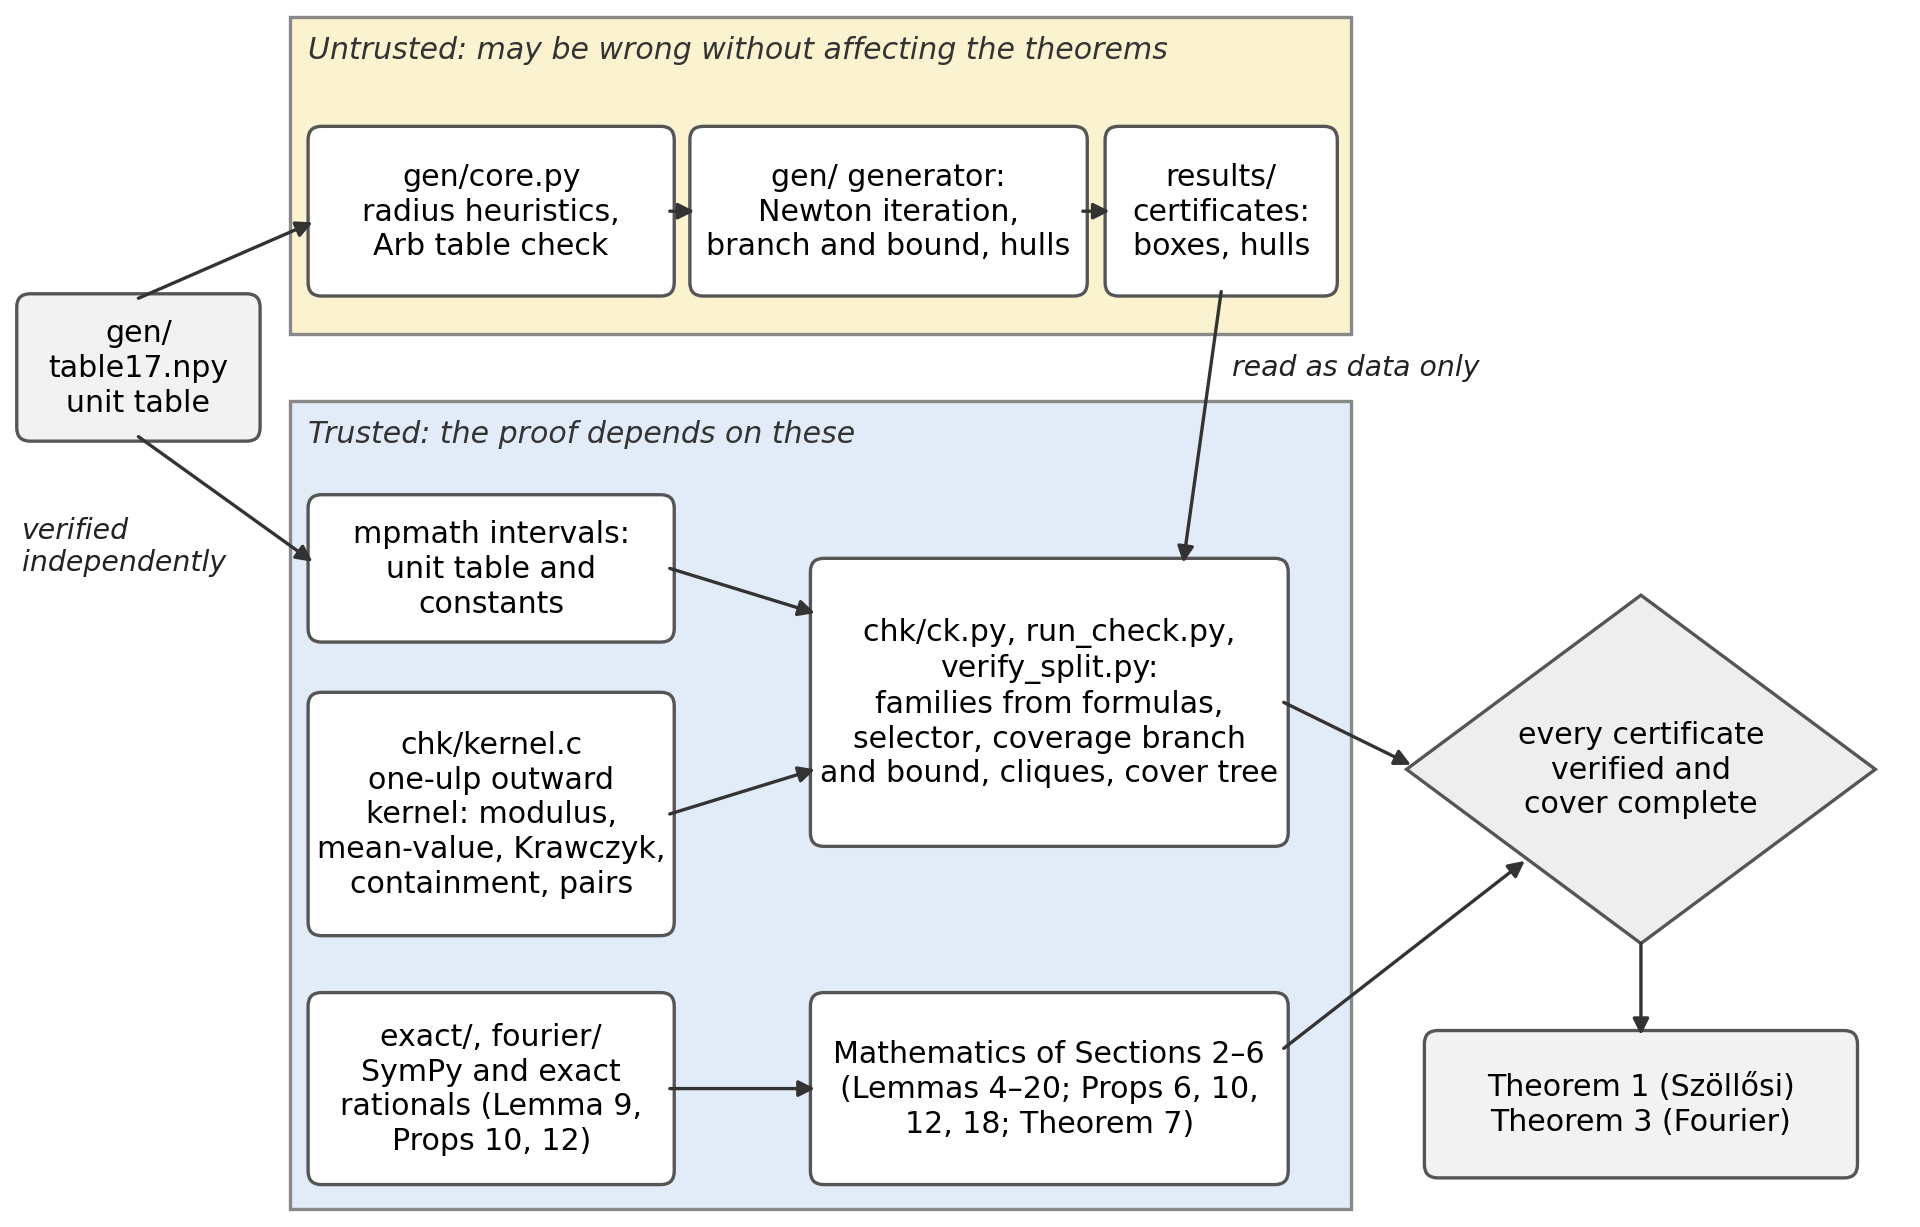
\includegraphics[width=1\linewidth,height=\textheight,keepaspectratio,alt={Data flow and trust. Theorems 1 and 3 depend only on the components in the lower (trusted) box; the generator may be wrong without affecting them, because every certificate it produces is re-verified by the checker.}]{fig_dependency.png}
\caption{Data flow and trust. Theorems 1 and 3 depend only on the
components in the lower (trusted) box; the generator may be wrong
without affecting them, because every certificate it produces is
re-verified by the checker.}
\end{figure}

\subsection{8.2 Independence boundaries}\label{independence-boundaries}

The referee asked for a precise statement of what each verification step
checks and what it shares with the main computation. Table 1 gives it.

{\def\LTcaptype{none} % do not increment counter
\begin{longtable}[]{@{}
  >{\raggedright\arraybackslash}p{(\linewidth - 4\tabcolsep) * \real{0.3333}}
  >{\raggedright\arraybackslash}p{(\linewidth - 4\tabcolsep) * \real{0.3333}}
  >{\raggedright\arraybackslash}p{(\linewidth - 4\tabcolsep) * \real{0.3333}}@{}}
\toprule\noalign{}
\begin{minipage}[b]{\linewidth}\raggedright
Question
\end{minipage} & \begin{minipage}[b]{\linewidth}\raggedright
Verified by
\end{minipage} & \begin{minipage}[b]{\linewidth}\raggedright
Shares with the generator
\end{minipage} \\
\midrule\noalign{}
\endhead
\bottomrule\noalign{}
\endlastfoot
Is the unit table correct to \(2^{-53}\) per component? & checker,
\texttt{mpmath.iv}, 40 digits & the table file (the object being
checked) \\
Does the selector keep the canonical owner of every point in
\(\mathcal F\)? & checker's selector (Lemma 11, Section 4.3) & nothing
(different formulas and arithmetic) \\
Is every kept box certified (cover completeness)? & checker's cover tree
(Lemma 20) & the list of certified boxes (checked data) \\
Do the hulls contain all unbiased vectors? & checker's coverage B\&B
(Proposition 18) & the hull end-points (checked data) \\
Are the hulls self-separated, and is (Cl) true? & checker's pair
intervals and set-based clique search & the hull end-points (checked
data) \\
Are the symmetry identities and fundamental domains correct? & SymPy and
exact rational scripts & nothing \\
\end{longtable}
}

Table 1. What is verified independently of the generator.

Here ``independent checker'' means implementation separation from the
generator. It does not mean independent human review or external
reproduction of every certificate. The supplied 30 September review
reports fresh graph checks for all certificates but fresh phase-space
replay for seven selected parents only. Its remaining phase-space
evidence was the submitted replay history.

\textbf{Replay binding (v3).} Each success now carries full SHA-256
binding to the family arrays, parameter indices and level, hull
endpoints, unit table, checker and subdivision sources, build script,
compiled kernel and runtime versions. Legacy or mismatched caches are
rejected. \texttt{-\/-clean} requires a new output and forbids
partial-run options; proof drivers disallow \texttt{MUB6\_KERNEL}.
Content hashes bind inputs but do not authenticate a dishonest cache
writer: the clean full replay imports no historical success records.
Explicit runtime checks replace assertions on the proof path, including
the family-installation call, so Python optimization cannot remove them.

The v3 regression suite retains the boundary-owner example, stale-cache
driver attack, changed-input binding tests and an exact generic
mixed-parameter Krawczyk fixture. The latter shows why dropping the
mixed term can falsely exclude a genuine root; it is not claimed to kill
the surviving mutation of the MUB kernel.

\subsection{8.3 Tests}\label{tests}

\emph{Checker test-suite} (\texttt{chk/tests/test\_kernel.py}, eleven
groups, all passing on both machines): T1 compares interval addition,
subtraction, multiplication, squaring and square roots with exact
rational arithmetic (\(16{,}052\) enclosures, including the referee's
value \(1+2^{-52}\), zeros, subnormals and the largest finite number);
T2 checks \(3{,}000\) enclosures of \(e^{i\varphi}\) over angle
intervals up to three full turns against 40-digit values; T3 checks
\(10{,}800\) rectangles for \(S_j\) at random points of random phase and
parameter boxes of both families; T4 submits \(373{,}188\) dyadic phase
boxes containing numerically converged solutions (residual below
\(10^{-10}\)) to the modulus, mean-value and Krawczyk tests, none of
which may exclude them; T5 samples pair values and checks the
self-separation bound and the orthogonality edges of the Fourier basis;
T6 checks that the selector keeps the boxes of \(5{,}465\) (point,
level) pairs of the fundamental domain, including \(\alpha=0\) and both
edges of the sector; T7 compares the containment test with brute-force
enumeration and with exact expectations for boxes whose end-points
coincide with, or lie one grid unit beyond, those of a hull, including
across the wrap-around (\(950\) decisions); T8 compares the exact
ordering test with brute-force enumeration over rational sub-grids; T9
compares the family data with the displayed formulas and checks the
Hadamard property on the constraint surface; T10 stresses the three
exclusion tests with coarse parameter boxes (levels \(3\)--\(7\)) and
non-dyadic phase boxes of widths \(1\) to \(1024\) grid units placed so
that a solution lies just inside a face (\(1{,}385{,}847\) boxes); T11
checks the Krawczyk assembly directly: for sampled vertices and interior
points \((w,q)\), the exactly evaluated point \((w-\tilde w)-YG(w;q)\)
must lie in the kernel's interval vector \(\mathcal K\) (\(2{,}880\)
points).

\emph{Mutation testing} (\texttt{chk/tests/mutate.py}; Jia and Harman
2011). The supplied record reports 16 of 17 kernel mutations detected by
the test suite. The survivor removes the mixed-parameter Jacobian term
in Lemma 17. This is incomplete test coverage, not evidence that the
term is unnecessary or impossible to test. The exact generic fixture
\(G(w;q)=(1+q)w-5/2\), \(W=[-1,1]\), \(Q=[0,2]\), \(\tilde w=0\),
\(c_Q=1\), \(Y=1/2\) has root \((w,q)=(5/6,2)\). Omitting the mixed term
gives \(\mathcal K=\{5/4\}\), falsely disjoint from \(W\); including it
gives \([3/4,7/4]\), containing the root. This permanent
rational-arithmetic test is not a claim to have killed the specific
MUB-kernel mutant.

\emph{Generator regression tests} (\texttt{tests/test\_gen.py})
reproduce each counterexample of the review and check the repair: the
disc product and the point--interval matrix product for \(r=1+2^{-52}\)
(also with zero left radius); \(20{,}000\) random disc products against
exact rational arithmetic; the cyclic-hull example and \(3{,}000\)
adversarial wrapping and nested cases; the referee's synthetic
``refined'' record, which is no longer counted as certified; and the
selector on sampled points of \(\mathcal F\) and on the special points
\(\alpha=0\), \(\alpha=1\) and the ray.

\emph{Historical platforms.} The submitted kernel test history records
three platforms (Section 9.1): x86-64 Linux with GCC 13.3, ARM64 Linux
with GCC 11.4, and ARM64 macOS with Apple clang 21. Those historical
logs report all groups passing; on the two platforms where the suite was
run in one piece (x86-64 Linux and macOS) every reported count is
identical. They do not establish a three-platform replay of the revised
Python drivers. The current local environment and fresh results are
recorded separately in the release receipt. On ARM64, compilers fuse
multiplications and additions by default; the explicit
\texttt{-ffp-contract=off} prevents this.

\section{9. The computations}\label{the-computations}

This section preserves the submitted generation and replay history and
its measured statistics. These historical machine runs are distinct from
the revised clean replay described in the release receipt. Historical
cache-based summaries are not by themselves verification of the revised
driver; the new release requires fresh input-bound coverage checks.

\subsection{9.1 Set-up}\label{set-up}

Three machines were used. \emph{Machine A} is a cloud virtual machine
(two Intel Xeon cores at 2.1 GHz, 8 GB, Ubuntu 24.04, Python 3.11, NumPy
2.4.4 with OpenBLAS, \texttt{mpmath} 1.3.0, \texttt{python-flint} 0.9.0,
GCC 13.3). \emph{Machine B} is an Apple M2 Mac mini (eight cores, 16 GB,
macOS, Python 3.14, NumPy 2.4.2, \texttt{mpmath} 1.3.0,
\texttt{python-flint} 0.9.0, Apple clang 21), shared with other work
during the run. \emph{Machine C} is an ARM64 Linux virtual machine on
the same Mac (Ubuntu 22.04, Python 3.10, NumPy 2.2.6, GCC 11.4), used
for the test-suite. BLAS threading was disabled in every process. The
unit table used by all runs has SHA-256
\texttt{075160008692331ecec57ebd851514642c5800b39d9bcad11c668c01074c5969};
it was verified by the generator with Arb and by the checker with
\texttt{mpmath}, independently, on each machine.

The Szöllősi roots (kept level-\(7\) boxes) were ordered by decreasing
\(|\alpha|\) at their centres. Machine A generated the certificates for
the roots at positions \(\equiv6\pmod7\) (195 roots, two processes);
machine B generated those at the other positions (six processes), except
the last \(250\) of its list, which machine A generated after finishing
its share. The Fourier certificates were generated on machine A. The
checker was run on machines A and B, each replaying part of the
certificates, and the final cover evaluation was run on the union of all
checker outputs.

\subsection{9.2 The Szöllősi family}\label{the-szuxf6llux151si-family-1}

The checker's selector keeps 160, 183, 232, 532, 1,367, 4,294 and 14,658
parameter boxes at levels \(3,\dots,9\); the 14,658 kept level-\(9\)
boxes lie below 1,088 of the 1,367 roots (the other roots have no kept
child). The generator certified every one of the 14,658 level-\(9\)
boxes at level \(9\) (12 of them in the second attempt with
\(L_{\max}=10\)); the only failed records are those of the incident
described in Section 9.4.

\emph{Historical checker replay.} The submitted checker history reports
all 14,658 certificates, 75 of them by parameter subdivision (Section
6.5) at parameter levels 10 to 12. Its cover evaluation, run on the
union of its outputs, reports every kept box of level \(3\) covered
(\texttt{chk\_results/chk\_szollosi\_summary.json}). For the revised
release, this historical summary is not the acceptance gate: Theorem 1
additionally requires the fresh input-bound full replay recorded in
\texttt{REPLAY\_RECEIPT.md}, together with the semantic arguments of
Theorem 7, Lemma 20 and Proposition 10.

The 75 boxes that needed parameter subdivision all contain parameters
with \(z=w=1\) (\(\theta_x+\theta_y\equiv\theta_u+\theta_v\equiv0\)),
where \(\alpha=1+2\cos\theta_x\) is real: they lie on the edge
\(\arg\alpha=0\) of the sector, with \(\alpha\) between about \(0.16\)
and the Diţă point \(\alpha=1\), and \(\theta_z,\theta_w\) sit at the
wrap-around point \(0\equiv2\pi\) of the ordering conditions. For 2 of
them no kept sub-box exists at the next level (the box does not meet
\(\mathcal F\)), so the verification is vacuous. For the others the
difficulty lies with the checker's first-order parametric Krawczyk test
on the full parameter box, not with the hulls: a numerical probe, which
is not part of the proof, sampled parameters on \(\Sigma\) in 4 of these
boxes and found all 60,864 numerically computed unbiased vectors inside
the stored hulls (\texttt{analysis/probe\_split\_boxes.log}).

Table 2 summarises the certificates. The number of numerically located
solutions, which only steers the grouping of boxes into hulls and is not
a certified count, is given as a complete histogram.

{\def\LTcaptype{none} % do not increment counter
\begin{longtable}[]{@{}
  >{\raggedright\arraybackslash}p{(\linewidth - 2\tabcolsep) * \real{0.5000}}
  >{\raggedright\arraybackslash}p{(\linewidth - 2\tabcolsep) * \real{0.5000}}@{}}
\toprule\noalign{}
\begin{minipage}[b]{\linewidth}\raggedright
quantity
\end{minipage} & \begin{minipage}[b]{\linewidth}\raggedright
value
\end{minipage} \\
\midrule\noalign{}
\endhead
\bottomrule\noalign{}
\endlastfoot
certified level-9 boxes (generator), replayed and verified (checker) &
14,658 / 14,658 \\
numerically located solutions per box (complete histogram, value: boxes)
& 42: 3; 48: 17; 49: 1; 54: 567; 55: 10; 56: 7; 57: 6; 58: 1; 59: 1; 60:
12,817; 63: 4; 64: 4; 72: 768; 84: 125; 96: 62; 108: 48; 120: 217 \\
boxes with rescued solutions; solutions rescued & 448; 5,229 \\
boxes with extra hulls from left-over clusters; extra hulls & 7,310;
40,247 \\
hulls per box: minimum, median, maximum & 0, 61, 141 \\
boxes without hulls & 2 \\
largest hull half-width per box: median, 99th percentile, maximum &
0.147, 0.233, 0.430 \\
six-cliques of \(O\) (checker): median and maximum per box; total & 9,
24303; 2,765,699 \\
edges of \(O\) and \(B\) (checker), maxima & 1,391, 4,493 \\
root-pass survivors at level 7 (checker): minimum, median, maximum &
1,778,718, 2,303,380, 7,177,859 \\
CPU time: generator, checker (hours) & 41.5, 15.4 \\
\end{longtable}
}

Table 2. Statistics of the Szöllősi certificates (generator) and of
their replay (checker).

The checker's coverage branch and bound needed phase levels up to 12
(the deepest level needed was 7 for 8 boxes, 8 for 2,407 boxes, 9 for
11,188 boxes, 10 for 1,040 boxes, 11 for 12 boxes, 12 for 1 box). The
total generator time was 42 CPU-hours and the checker time 15 CPU-hours.

\emph{Special parameters.} At the special parameters: the box (0, 170,
0, 170) containing \(\alpha=0\) was verified directly, with 49 hulls (60
numerical solutions, largest hull half-width 0.172); its graph \(O\) has
212 edges and 60 six-cliques and \(B\) has 451 edges; the box (19, 137,
203, 322) containing the ray point
\(\alpha=\tfrac12+\tfrac{i}{2\sqrt3}\) was verified directly, with 54
hulls (54 numerical solutions, largest hull half-width 0.160); its graph
\(O\) has 112 edges and 1 six-clique and \(B\) has 336 edges; the box
(0, 128, 0, 256) containing the Diţă point \(\alpha=1\) was verified
directly, with 120 hulls (120 numerical solutions, largest hull
half-width 0.098); its graph \(O\) has 826 edges and 10 six-cliques and
\(B\) has 2,710 edges. In each case no six-clique of \(O\) has a partner
clique across \(B\).

\subsection{9.3 The Fourier family}\label{the-fourier-family-1}

The selector of Section 4.3 keeps 3, 5, 15, 41, 143, 505 and 1,935 boxes
at levels \(3,\dots,9\). The generator certified all 1,935 level-\(9\)
boxes at level \(9\), and the checker verified all of them; its cover
evaluation is complete
(\texttt{chk\_results/chk\_fourier\_summary.json}). By Theorem 7 and
Proposition 12 this proves Theorem 3.

The certificates agree with the numerical observations of Jaming et al.,
which they do not depend on. In every box the generator located 48
unbiased vectors numerically (their Numerical Evidence 1.3: \(48\) for
all \((a,b)\)). The six-cliques of the graph \(O\) are the candidate
orthonormal bases: in 1,876 of the 1,935 boxes there are exactly \(8\)
of them (their observation for generic parameters), in the box at
\((a,b)=(0,0)\) there are 16 (they report \(16\) bases for \(F_6\)), and
in the box containing \((a,b)=(1/6,0)\) there are exactly 70 (they
report \(70\)). The largest number, 897, occurs in the neighbouring box
(84, 0), where hulls of nearby vectors overlap.

{\def\LTcaptype{none} % do not increment counter
\begin{longtable}[]{@{}
  >{\raggedright\arraybackslash}p{(\linewidth - 2\tabcolsep) * \real{0.5000}}
  >{\raggedright\arraybackslash}p{(\linewidth - 2\tabcolsep) * \real{0.5000}}@{}}
\toprule\noalign{}
\begin{minipage}[b]{\linewidth}\raggedright
quantity
\end{minipage} & \begin{minipage}[b]{\linewidth}\raggedright
value
\end{minipage} \\
\midrule\noalign{}
\endhead
\bottomrule\noalign{}
\endlastfoot
certified level-9 boxes (generator), replayed and verified (checker) &
1,935 / 1,935 \\
numerically located solutions per box & 48: 1,935 \\
hulls per box: minimum, median, maximum & 48, 48, 55 \\
largest hull half-width per box: median, maximum & 0.049, 0.172 \\
six-cliques of \(O\) (checker): median and maximum per box & 8, 897 \\
deepest phase level in the checker (level: boxes) & 8: 74; 9: 1,858; 10:
3 \\
CPU time: generator, checker (hours) & 0.48, 0.38 \\
\end{longtable}
}

Table 3. Statistics of the Fourier certificates and their historical
replay.

\subsection{9.4 History of the run}\label{history-of-the-run}

Three incidents are recorded because the raw results files contain their
traces; none of them touches the checker, and every record written in
these circumstances is either a certificate, which the checker verifies
like any other, or a failed or refined record, which is not used.

First, machine B's Python installation lacked SciPy, which the generator
used for the connected components that group left-over boxes into extra
hulls. The resulting exceptions were treated, correctly, as failed
certificates, and the affected level-\(9\) boxes were subdivided down to
level \(12\), where 860 records ended in the state \emph{failed}. The
component routine was replaced by a SciPy-free union--find in NumPy
(tested against SciPy on \(300\) random graphs), the run was resumed,
and every affected level-\(9\) box was then certified at level \(9\);
the checker's cover tree stops at those certificates.

Second, machine B's generator was restarted twice: once with a limit on
its list of roots, to hand the last \(250\) roots to machine A, and once
for the repair just described. The resumption logic skipped every box
already certified. On macOS the worker processes of an interrupted run
are not terminated with their parent, and those of one interrupted run
continued for about half an hour, appending records, before they were
found and stopped.

Third, machine A's container was restarted by its host during the tail
run, which then resumed from its results file.

\subsection{9.5 Relation to the earlier
computation}\label{relation-to-the-earlier-computation}

The earlier computation certified \(15{,}648\) level-\(9\) boxes
selected by the non-rigorous selector; the rigorous selector keeps
\(14{,}658\), all of them among the earlier ones. None of the earlier
certificates is used. As a test of the checker's strength on the hardest
parameters, it was also applied to six earlier certificates near
\(\alpha=0\), on the ray and near \(\alpha=1\), and verified all of
them.

\section{10. Numerical diagnostics of degenerate
parameters}\label{numerical-diagnostics-of-degenerate-parameters}

This section reports numerical observations that are \textbf{not part of
the proof}; the certificate needs neither their correctness nor any
statement about the structure of \(\mathcal U(H)\). The earlier version
described coalescing unbiased vectors on the ray \(\arg\alpha=\pi/6\)
and at \(\alpha=0\) as coinciding ``exactly'' and as not isolated; the
referee pointed out that nearby clustering and small singular values do
not distinguish an isolated multiple root from a positive-dimensional
component. The observations below are therefore stated as diagnostics,
computed in \(60\)-digit arithmetic
(\texttt{exact/degeneracy\_diagnostics.py}): solutions were located by
multistart Newton iteration in binary64 (\(40{,}000\) starts), refined
by damped Gauss--Newton iteration in \texttt{mpmath} until the residual
of all six equations was below \(10^{-40}\), and de-duplicated at
distance \(10^{-18}\); for each refined solution the singular values of
the \(6\times5\) real Jacobian were computed. A singular value below
\(10^{-20}\) is reported as ``numerically singular''.

{\def\LTcaptype{none} % do not increment counter
\begin{longtable}[]{@{}
  >{\raggedright\arraybackslash}p{(\linewidth - 10\tabcolsep) * \real{0.1364}}
  >{\raggedleft\arraybackslash}p{(\linewidth - 10\tabcolsep) * \real{0.1818}}
  >{\raggedleft\arraybackslash}p{(\linewidth - 10\tabcolsep) * \real{0.1818}}
  >{\raggedleft\arraybackslash}p{(\linewidth - 10\tabcolsep) * \real{0.1818}}
  >{\raggedleft\arraybackslash}p{(\linewidth - 10\tabcolsep) * \real{0.1818}}
  >{\raggedright\arraybackslash}p{(\linewidth - 10\tabcolsep) * \real{0.1364}}@{}}
\toprule\noalign{}
\begin{minipage}[b]{\linewidth}\raggedright
parameter \(\alpha\)
\end{minipage} & \begin{minipage}[b]{\linewidth}\raggedleft
distinct solutions
\end{minipage} & \begin{minipage}[b]{\linewidth}\raggedleft
numerically singular
\end{minipage} & \begin{minipage}[b]{\linewidth}\raggedleft
smallest singular value (others)
\end{minipage} & \begin{minipage}[b]{\linewidth}\raggedleft
minimal distance
\end{minipage} & \begin{minipage}[b]{\linewidth}\raggedright
clusters (linkage \(\le10\delta\))
\end{minipage} \\
\midrule\noalign{}
\endhead
\bottomrule\noalign{}
\endlastfoot
\(0.7+0.1i\) (generic) & 60 & 0 & \(0.84\) & \(0.33\) & --- \\
\(1\) (boundary, Diţă) & 120 & 0 & \(1.11\) & \(0.71\) & --- \\
ray, \(\delta=10^{-2}\) & 60 & 0 & \(1.9\cdot10^{-2}\) &
\(7.5\cdot10^{-3}\) & two of size 4 \\
ray, \(\delta=10^{-4}\) & 60 & 0 & \(1.9\cdot10^{-4}\) &
\(7.5\cdot10^{-5}\) & two of size 4 \\
\(\tfrac12+\tfrac{i}{2\sqrt3}\) (on the ray) & 54 & 2 & \(1.25\) &
\(0.67\) & --- \\
near \(0\), \(\delta=10^{-2}\) & 60 & 0 & \(9.0\cdot10^{-3}\) &
\(3.45\cdot10^{-3}\) & six of size 4 \\
near \(0\), \(\delta=10^{-4}\) & 60 & 0 & \(9.0\cdot10^{-5}\) &
\(3.45\cdot10^{-5}\) & six of size 4 \\
\(0\) & 42 & 6 & \(3.0\) & \(1.32\) & --- \\
\end{longtable}
}

Table 4. Unbiased vectors at special parameters. Distances are
\(\max_k|e^{i\theta_k}-e^{i\phi_k}|\); clusters are single-linkage
clusters at that distance. ``Ray, \(\delta\)'' is
\(\alpha=3^{-1/2}e^{i(\pi/6-\delta)}\) and ``near \(0\), \(\delta\)'' is
\(\alpha=\delta e^{i\pi/12}\). The exact point of the ray is
\(\alpha=\tfrac12+\tfrac{i}{2\sqrt3}=3^{-1/2}e^{i\pi/6}\) (the earlier
version gave the decimal approximation \(0.5+0.2887i\)).

The pattern is consistent across the table. Approaching the ray, two
groups of four solutions contract linearly in \(\delta\), and the
smallest singular value of the Jacobian at their members decreases
linearly as well; at the exact ray point \(54\) distinct solutions are
found, \(52\) with well-conditioned Jacobians and \(2\) at which the
Jacobian is numerically singular, which is what one expects if each
group of four converges to a single singular solution
(\(52+2\cdot4=60\)). Approaching \(\alpha=0\), six groups of four
contract in the same way, and at \(\alpha=0\) there are \(42=36+6\)
distinct solutions, \(6\) of them numerically singular. At the smallest
separations tried (\(\delta=10^{-6}\)) the binary64 multistart no longer
resolves all members of the groups (it finds \(56\) and \(50\) solutions
respectively), which illustrates the difficulty faced by a certificate
that isolates simple roots: at any fixed resolution there are parameters
near these loci at which members of a group are closer together than the
resolution, and a simple-root isolation test (such as the Krawczyk test
used here, applied to single boxes) cannot succeed on a box containing
two of them. The present certificate avoids the question by enclosing
whole groups in single hulls. Whether the singular solutions are
isolated multiple roots or points of positive-dimensional components is
not decided by these computations and is not needed.

\section{11. Discussion}\label{discussion}

\subsection{11.1 What has been proved}\label{what-has-been-proved}

Theorem 1 settles Conjecture 3 of MMVW for every complex Hadamard matrix
of the two-circulant form (4.2), that is, for every \(\alpha\) in the
closed region \(\mathbb D\), boundary and degenerate loci included. With
Theorem 3 (Jaming et al.'s result, re-proved here), both families that
appear in MMVW's Proposition 4.2 are now excluded by certificates
verified by the same checker, so that MMVW's route to Zauner's
conjecture in dimension six depends only on their Conjecture 2. Theorem
1 says nothing about Conjecture 2, nor about complex Hadamard matrices
outside the two families. The classification of complex Hadamard
matrices of order six announced by Cárdenes Wuttig and Tindall (2026) is
a statement about Hadamard matrices, not about mutually unbiased bases,
and is not used.

\subsection{11.2 Comparison with Jaming et
al.~(2009)}\label{comparison-with-jaming-et-al.-2009}

Jaming et al.~replaced the parameters by the centres of \(N=180\) cells
per unit of \(a\) and \(b\) (\(270\) cells for the fundamental triangle)
and the phases of candidate vectors by the centres of \(N'=19\) cells
per turn, refined dyadically for seven generations. Their Lemma 3.1 (the
``trivial error bound'') and Lemma 3.2 (the maximal deviation of an
inner-product sum over a product of small intervals is attained at
end-points) give explicit conditions that a cell must satisfy if it
contains a vector unbiased to \(F(a,b)\) or orthogonal to another; an
exhaustive search over the surviving ``quasi-unbiased'' vectors then
showed that no two ``\(N'\)-orthonormal'' bases that are
``\(N'\)-unbiased'' to each other exist. The program ran for about six
hours. The argument has the same three components as ours --- a
parameter cover, an enclosure of the unbiased vectors per cell, and a
combinatorial exclusion --- and MMVW rightly regarded it as the template
for Conjecture 3. The present work differs in the following respects,
which are the improvements it claims.

\begin{itemize}
\tightlist
\item
  \emph{Rounding.} This package supplies a separate outward-rounded
  checker, a verified unit table and explicitly checked constants. We do
  not make an implementation-specific criticism of the historical
  program without an archived source snapshot. The published 2009
  mathematical theorem remains the predecessor being re-proved, not an
  unproved claim.
\item
  \emph{Exclusion strength.} Their cell tests are of order zero: they
  bound how far the inner-product sums can move within a cell, without
  derivative information, so that a cell can be discarded only once it
  is small compared with its distance from the solution set. Ours add a
  mean-value test and a parametric Krawczyk test, both using derivatives
  with respect to the phases and the parameters, so that for parameter
  cells of width \(2\pi/2^9\) the phase-space subdivision stops at level
  \(9\) or \(10\) even close to solutions.
\item
  \emph{Clusters.} Near degenerate parameters the unbiased vectors of
  the Szöllősi family coalesce (Section 10). The certificate does not
  need to separate them: a hull may contain a cluster, and the
  self-separation condition is all that the combinatorial step requires.
  The Fourier family has no such loci in its triangle, which is
  consistent with the absence of any special treatment in Jaming et al.
\item
  \emph{Verification design.} The certificates are produced by one
  program and verified by another, with a small trusted kernel and an
  explicit list of what the proof depends on (Section 8).
\item
  \emph{Transferability.} The Fourier family was handled by the same
  generator and checker as the Szöllősi family; the family-specific
  inputs were the exponent data, the coefficient rectangles and the
  selector.
\end{itemize}

\subsection{11.3 Assumptions and limits}\label{assumptions-and-limits}

The trusted components are listed in Section 8.1. The mathematics is not
formalised in a proof assistant. Mutation coverage is incomplete: one
supplied kernel mutation survived. Lemma 17 and the exact generic
assembly fixture demonstrate the mixed term's necessity, but the fixture
is not a kernel-specific mutation kill. The certificate does not assume
that numerical root discoveries are complete or that \(\mathcal U(H)\)
is finite. Exact identities and finite checks retain their stated scope;
neither producer-side replay nor model review establishes external peer
review.

\subsection{11.4 Transfer to other
families}\label{transfer-to-other-families}

The implemented interface accepts entries that are unimodular constants
times torus characters, with the specified trigonometric constraint
structure. Transfer has been demonstrated only for the two families in
this paper and their equivalences. Karlsson's three-parameter family and
Szöllősi's four-parameter family are research directions, not
established inputs to this checker. Their algebraic reconstruction,
denominators, branch choices and exceptional cases require complete
encodings and coverage proofs. The present kernel has capacities
\texttt{MAXP=4}, \texttt{MAXT=8} and \texttt{MAXN=7}; an enlarged
encoding could require kernel changes and renewed verification.
Parameter counts alone do not prove compatibility, and no exclusion for
either larger family is claimed.

\subsection{11.5 Availability and
disclosure}\label{availability-and-disclosure}

The release package provides the source, certificates, checker, replay
records and a machine-oriented index. The scholarly attribution is
Anonymous. The supplied manuscript credited Claude; Codex performed the
present revision and publication checks. These are reported system
roles, not externally audited authorship or human peer review. No human
mathematical contribution is inferred from account ownership. Funding
and conflicts were not recorded in the supplied research provenance;
none are inferred. This is mathematical research without human-subject
data. Original research contents are CC0-1.0 and original code is MIT,
with third-party exceptions listed in \texttt{LICENSES.md}.

\section{Appendix A. Withdrawn generator rounding
claim}\label{appendix-a.-withdrawn-generator-rounding-claim}

The generator is outside the trusted computing base. The former Lemma R
and its proof are withdrawn: multiplication combines uncertainty from
both operands, invalidating the claimed intermediate induction. With
\(u=2^{-53}\), two exact inputs \((1-u)^{-8}\) represented by computed
values \(1\) have product \((1-u)^{-16}\), exceeding the asserted
exponent \(9\) even with its small additive allowance. This does not
refute the final padded bound, but that unused bound is no longer
claimed. The padding rule below remains a generator heuristic; every
proposal must be checked independently.

The implemented rule is
\(\mathrm{up}(x)=\mathrm{fl}(\mathrm{fl}(x(1+2^{-40}))+2^{-800})\).

Generator regression tests are diagnostics, not proof of a general
rounding lemma. The theorem relies on the separate outward-rounded
checker, not these heuristics.

Every radius returned by a generator primitive is passed through
\(\mathrm{up}\) (and replaced by \(+\infty\) if it exceeds \(2^{64}\) or
is not a number); differences and lower bounds are formed by a single
correctly rounded operation on exact operands followed by a one-ulp
step, as in Lemma 13; and all exclusion decisions are strict comparisons
of a lower bound with an upper bound, which are false whenever a NaN or
infinity occurs.

\section{Appendix B. Response to the second
review}\label{appendix-b.-response-to-the-second-review}

This revision responds to the 30 September 2026 review of version 2.
Historical logs remain evidence of the submitted version, not fresh
verification of the revised driver.

{\def\LTcaptype{none} % do not increment counter
\begin{longtable}[]{@{}
  >{\raggedright\arraybackslash}p{(\linewidth - 2\tabcolsep) * \real{0.5000}}
  >{\raggedright\arraybackslash}p{(\linewidth - 2\tabcolsep) * \real{0.5000}}@{}}
\toprule\noalign{}
\begin{minipage}[b]{\linewidth}\raggedright
Obligation
\end{minipage} & \begin{minipage}[b]{\linewidth}\raggedright
Disposition
\end{minipage} \\
\midrule\noalign{}
\endhead
\bottomrule\noalign{}
\endlastfoot
Closed enclosures versus half-open ownership & Theorem 7, Lemma 11 and
Lemma 20 now use canonical half-open owners. Direct interval tests use
closed enclosures; subdivision covers the retained fundamental-domain
portion. The explicit boundary counterexample is retained as a
regression. \\
Cache accepts changed hulls & Receipts bind the actual hulls, family,
table, checker sources, compiled kernel and runtime. Legacy and
mismatched receipts are rejected. Clean replay starts with no receipts;
proof drivers reject kernel overrides. The stale-cache attack is an
executable negative control. \\
Python optimization & A further defect found during revision placed the
family-installation call inside an assertion. This is now an explicit
runtime call; optimized-Python regression tests exercise it. \\
Unsupported larger-family transfer & Section 11.4 treats larger Karlsson
and Szöllősi families as future work, with finite torus-character
capacities and additional algebraic-branch obligations. \\
Invalid generator-rounding induction & Appendix A withdraws the unused
lemma and explains the exponent error. Generator padding is not part of
the proof; checker containment remains necessary. \\
Mixed-parameter Krawczyk term & An exact generic example demonstrates
false exclusion if the term is omitted. This is not a claim to kill the
surviving MUB-kernel mutation. \\
Subdivision depth & The account includes all eight historical
depth-three parents and the maximum permitted level 12. \\
Historical numerical-code comparison & Unsupported implementation
criticism has been removed. The Fourier precedent is credited as an
existing theorem, not a new result. \\
Assurance and counts & Numerical solution counts, hull counts, graph
checks and phase-space replay are distinguished. The supplied reviewer
checked all graphs but only selected phase-space parents afresh.
Implementation separation is not external peer review. \\
Reusable interface & A standalone certificate-interface description
states ownership, arithmetic, coverage and graph obligations.
Larger-family encoding and formalization remain optional future work,
not achievements of this package. \\
\end{longtable}
}

The release replay receipt, rather than historical per-machine
summaries, determines the verification status of this revision.

\section{Appendix C. Inventory of code and
data}\label{appendix-c.-inventory-of-code-and-data}

Line counts and SHA-256 digests (first 16 hexadecimal digits) of the
files on which the results depend; the bundle file \texttt{SHA256SUMS}
lists the full digests of every file, including all results, checker
outputs and logs.

\textbf{Checker (trusted)}

{\def\LTcaptype{none} % do not increment counter
\begin{longtable}[]{@{}lrl@{}}
\toprule\noalign{}
file & lines & SHA-256 (prefix) \\
\midrule\noalign{}
\endhead
\bottomrule\noalign{}
\endlastfoot
\texttt{chk/kernel.c} & 638 & \texttt{9214d0d935ad21a4} \\
\texttt{chk/ck.py} & 385 & \texttt{b134fbef3bae0b90} \\
\texttt{chk/run\_check.py} & 162 & \texttt{382b7910b5195adc} \\
\texttt{chk/verify\_split.py} & 77 & \texttt{8ba748ea3e78101e} \\
\texttt{chk/receipt\_binding.py} & 58 & \texttt{45ade521a0d9173d} \\
\texttt{chk/full\_replay.py} & 55 & \texttt{556b31cae41a8769} \\
\texttt{chk/build.sh} & 11 & \texttt{fcdb7df0fe374ff1} \\
\end{longtable}
}

\textbf{Exact verification (trusted)}

{\def\LTcaptype{none} % do not increment counter
\begin{longtable}[]{@{}lrl@{}}
\toprule\noalign{}
file & lines & SHA-256 (prefix) \\
\midrule\noalign{}
\endhead
\bottomrule\noalign{}
\endlastfoot
\texttt{exact/lemma5\_exact.py} & 111 & \texttt{e8142d5eb38c242f} \\
\texttt{fourier/symmetries.py} & 129 & \texttt{837092d6674b4a0a} \\
\texttt{fourier/fundamental\_domain.py} & 111 &
\texttt{1913323ee3ebb240} \\
\texttt{fourier/fourier\_exact.py} & 17 & \texttt{6c64edd26c29f8c2} \\
\end{longtable}
}

\textbf{Tests}

{\def\LTcaptype{none} % do not increment counter
\begin{longtable}[]{@{}lrl@{}}
\toprule\noalign{}
file & lines & SHA-256 (prefix) \\
\midrule\noalign{}
\endhead
\bottomrule\noalign{}
\endlastfoot
\texttt{chk/tests/test\_kernel.py} & 408 & \texttt{1d55f31c282ccb07} \\
\texttt{chk/tests/test\_revision.py} & 63 & \texttt{83dfeefc5abcdd6b} \\
\texttt{chk/tests/test\_boundary\_interval.py} & 40 &
\texttt{67470e36835c335d} \\
\texttt{chk/tests/mutate.py} & 57 & \texttt{6f504b9dfbb59629} \\
\texttt{tests/test\_gen.py} & 91 & \texttt{5806d6e653e7ffec} \\
\end{longtable}
}

\textbf{Generator (untrusted)}

{\def\LTcaptype{none} % do not increment counter
\begin{longtable}[]{@{}lrl@{}}
\toprule\noalign{}
file & lines & SHA-256 (prefix) \\
\midrule\noalign{}
\endhead
\bottomrule\noalign{}
\endlastfoot
\texttt{gen/rnd.py} & 63 & \texttt{b5b23bec4e1cecff} \\
\texttt{gen/family.py} & 87 & \texttt{ceca8f8526730917} \\
\texttt{gen/core.py} & 320 & \texttt{45e90739fa9de956} \\
\texttt{gen/hulls.py} & 116 & \texttt{788317275e06297f} \\
\texttt{gen/comb.py} & 73 & \texttt{bff994877171e98f} \\
\texttt{gen/selector.py} & 104 & \texttt{eed4a8ade8ea638b} \\
\texttt{gen/solve.py} & 197 & \texttt{c692cdcf00c7fad7} \\
\texttt{gen/driver.py} & 131 & \texttt{cd4fd20bdb3215b3} \\
\texttt{gen/helpers\_v2.py} & 12 & \texttt{ca1ba100a1baec90} \\
\end{longtable}
}

\textbf{Diagnostics and analysis (not part of the proof)}

{\def\LTcaptype{none} % do not increment counter
\begin{longtable}[]{@{}lrl@{}}
\toprule\noalign{}
file & lines & SHA-256 (prefix) \\
\midrule\noalign{}
\endhead
\bottomrule\noalign{}
\endlastfoot
\texttt{exact/degeneracy\_diagnostics.py} & 145 &
\texttt{0169911f82c81913} \\
\texttt{analysis/stats.py} & 102 & \texttt{c64b1811f6ac85d9} \\
\texttt{analysis/empty\_boxes.py} & 31 & \texttt{6663ceeddaa6f7bf} \\
\texttt{analysis/ready\_roots.py} & 23 & \texttt{c454da242201d947} \\
\texttt{analysis/probe\_split\_boxes.py} & 44 &
\texttt{0f4c9d23bf6ea7cc} \\
\texttt{analysis/special\_boxes.py} & 23 & \texttt{082156ef59bb789f} \\
\end{longtable}
}

\textbf{Data}

{\def\LTcaptype{none} % do not increment counter
\begin{longtable}[]{@{}lrl@{}}
\toprule\noalign{}
file & lines & SHA-256 (prefix) \\
\midrule\noalign{}
\endhead
\bottomrule\noalign{}
\endlastfoot
\texttt{gen/table17.npy} & --- & \texttt{075160008692331e} \\
\end{longtable}
}

Totals: checker (trusted), 1386 lines; exact verification (trusted), 368
lines; tests, 659 lines; generator (untrusted), 1103 lines; diagnostics
and analysis (not part of the proof), 368 lines.

\emph{Version boundary.} These hashes describe revised source.
Historical logs refer to earlier versions and are not fresh receipts for
these bytes. Revised clean-replay summaries bind their exact sources,
compiled kernel, certificate inputs and environment. Generator
variations cannot replace checker verification.

\section{Sources}\label{sources}

Sources are grouped by theme; URLs are given for every item.

\textbf{The conjecture and its context}

Matolcsi, M., Matszangosz, Á. K., Varga, D., \& Weiner, M. (2025).
\emph{Triplets of mutually unbiased bases} (arXiv:2503.14752v2)
{[}Preprint{]}. arXiv. \url{https://arxiv.org/abs/2503.14752} (version 2
of 19 July 2025 consulted: Conjecture 3 and Proposition 4.2, p.~16)

Matolcsi, M., Matszangosz, Á. K., Varga, D., \& Weiner, M. (2026).
Triplets of mutually unbiased bases. \emph{Journal of Algebraic
Combinatorics, 63}, Article 26.
\url{https://doi.org/10.1007/s10801-026-01506-x}

Chen, X., Liang, M., Hu, M., \& Chen, L. (2021). \(H_2\)-reducible
matrices in six-dimensional mutually unbiased bases. \emph{Quantum
Information Processing, 20}, Article 353.
\url{https://doi.org/10.1007/s11128-021-03278-8}

McNulty, D., \& Weigert, S. (2025). \emph{Comment on ``Product states
and Schmidt rank of mutually unbiased bases in dimension six''}
(arXiv:2504.13067) {[}Preprint{]}. arXiv.
\url{https://arxiv.org/abs/2504.13067}

Liang, M., \& Chen, L. (2025; version 3 updated 24 August 2026).
\emph{Reply to Comment on ``Product states and Schmidt rank of mutually
unbiased bases in dimension six''} (arXiv:2504.15576v3) {[}Preprint{]}.
arXiv. \url{https://arxiv.org/abs/2504.15576v3}

McNulty, D., \& Weigert, S. (2026). Mutually unbiased bases in composite
dimensions --- A review. \emph{Quantum, 10}, 2051.
\url{https://doi.org/10.22331/q-2026-04-01-2051} (preprint:
\url{https://arxiv.org/abs/2410.23997})

Zauner, G. (2011). Quantum designs: Foundations of a noncommutative
design theory. \emph{International Journal of Quantum Information,
9}(1), 445--507. \url{https://doi.org/10.1142/S0219749911006776}

\textbf{Families of complex Hadamard matrices and the discretisation
technique}

Szöllősi, F. (2010). A two-parameter family of complex Hadamard matrices
of order 6 induced by hypocycloids. \emph{Proceedings of the American
Mathematical Society, 138}(3), 921--928.
\url{https://doi.org/10.1090/S0002-9939-09-10102-8} (preprint:
\url{https://arxiv.org/abs/0811.3930})

Szöllősi, F. (2012). Complex Hadamard matrices of order 6: A
four-parameter family. \emph{Journal of the London Mathematical Society,
85}(3), 616--632. Preprint: \url{https://arxiv.org/abs/1008.0632}

Karlsson, B. R. (2011). Three-parameter complex Hadamard matrices of
order 6. \emph{Linear Algebra and its Applications, 434}(1), 247--258.
\url{https://doi.org/10.1016/j.laa.2010.08.020}

Bengtsson, I., Bruzda, W., Ericsson, Å., Larsson, J.-Å., Tadej, W., \&
Życzkowski, K. (2007). Mutually unbiased bases and Hadamard matrices of
order six. \emph{Journal of Mathematical Physics, 48}(5), 052106.
\url{https://arxiv.org/abs/quant-ph/0610161}

Jaming, P., Matolcsi, M., Móra, P., Szöllősi, F., \& Weiner, M. (2009).
A generalized Pauli problem and an infinite family of MUB-triplets in
dimension 6. \emph{Journal of Physics A: Mathematical and Theoretical,
42}(24), 245305. \url{https://doi.org/10.1088/1751-8113/42/24/245305}
(preprint: \url{https://arxiv.org/abs/0902.0882})

Jaming, P., Matolcsi, M., Móra, P., Szöllősi, F., \& Weiner, M. (2009).
\emph{Documentation of results} (programs \texttt{ort.cpp} and
\texttt{fab\_ubv.cpp}, output \texttt{fab\_ubv.txt}) {[}Computer
software and data{]}.
\url{http://www.math.bme.hu/~matolcsi/angpubl.html}

Cárdenes Wuttig, M., \& Tindall, J. (2026). \emph{A complete
classification of complex Hadamard matrices of order six}
(arXiv:2608.18053v2) {[}Preprint{]}. arXiv.
\url{https://arxiv.org/abs/2608.18053}

\textbf{Verified computation and software}

Institute of Electrical and Electronics Engineers. (2019). \emph{IEEE
standard for floating-point arithmetic} (IEEE Std 754-2019).
\url{https://doi.org/10.1109/IEEESTD.2019.8766229}

Krawczyk, R. (1969). Newton-Algorithmen zur Bestimmung von Nullstellen
mit Fehlerschranken. \emph{Computing, 4}(3), 187--201.
\url{https://doi.org/10.1007/BF02234767}

Neumaier, A. (1990). \emph{Interval methods for systems of equations}.
Cambridge University Press.
\url{https://doi.org/10.1017/CBO9780511526473}

Higham, N. J. (2002). \emph{Accuracy and stability of numerical
algorithms} (2nd ed.). SIAM.
\url{https://doi.org/10.1137/1.9780898718027}

Jia, Y., \& Harman, M. (2011). An analysis and survey of the development
of mutation testing. \emph{IEEE Transactions on Software Engineering,
37}(5), 649--678. \url{https://doi.org/10.1109/TSE.2010.62}

Johansson, F. (2017). Arb: Efficient arbitrary-precision midpoint-radius
interval arithmetic. \emph{IEEE Transactions on Computers, 66}(8),
1281--1292. \url{https://doi.org/10.1109/TC.2017.2690633}

Johansson, F., et al.~(2023). \emph{mpmath: A Python library for
arbitrary-precision floating-point arithmetic} (Version 1.3.0)
{[}Computer software{]}. \url{https://mpmath.org/}

Meurer, A., Smith, C. P., Paprocki, M., Čertík, O., Kirpichev, S. B.,
Rocklin, M., \ldots{} Scopatz, A. (2017). SymPy: Symbolic computing in
Python. \emph{PeerJ Computer Science, 3}, e103.
\url{https://doi.org/10.7717/peerj-cs.103}

Harris, C. R., Millman, K. J., van der Walt, S. J., Gommers, R.,
Virtanen, P., Cournapeau, D., \ldots{} Oliphant, T. E. (2020). Array
programming with NumPy. \emph{Nature, 585}, 357--362.
\url{https://doi.org/10.1038/s41586-020-2649-2}

The python-flint developers. (2025). \emph{python-flint: Python bindings
for FLINT and Arb} (Version 0.9.0) {[}Computer software{]}.
\url{https://github.com/flintlib/python-flint}

\textbf{Review of the earlier version}

Anonymous referee. (2026, September 29). \emph{Review: Szöllősi-family
MUB exclusion} {[}Unpublished referee report of the earlier bundle
\texttt{mub6\_szollosi\_conjecture3.zip} (SHA-256 prefix
944044376cda648e), with the reproducible audit bundle
\texttt{mub6\_referee\_audit\_2026-09-29.zip} (SHA-256 prefix
a4d08188e57262eb){]}. Both are included in the bundle accompanying this
paper (directory \texttt{review/}).

\end{document}
